\documentclass[utf8]{frontiersSCNS} % for Scsence, Engineering and Humanities and Social Sciences articles
% \documentclass[utf8]{frontiersFPHY} % for Physics and Applied Mathematics and Statistics articles
\usepackage{gensymb}
\usepackage{url,hyperref,lineno,microtype,subcaption}
\usepackage[onehalfspacing]{setspace}

\usepackage{tabularx}
\linenumbers
\DeclareUnicodeCharacter{0301}{}
\DeclareUnicodeCharacter{2212}{}
\usepackage{wasysym} % provides \DH, \dh, \Thorn, \thorn
% Leave a blank\usepackage{amsmath}
%\DeclareMathOperator{\sign}{sign} line between paragraphs instead of using \\

% \usepackage{csvsimple} % for csv tables
\usepackage{booktabs}
\usepackage{multirow}

\def\keyFont{\fontsize{8}{11}\helveticabold }
\def\firstAuthorLast{Balasubramanian {et~al.}} %use et al only if is more than 1 author
\def\Authors{Suryanarayanan Balasubramanian\,$^{1*,3}$, Martin Hoelzle\,$^{1}$, Michael Lehning\,$^{2}$, Jordi
	Bolibar\,$^{4}$, Sonam Wangchuk\,$^{3}$, Johannes Oerlemans\,$^{4}$, and Felix Keller\,$^{5,6}$}
\def\Address{$^{1}$University of Fribourg, Fribourg, Switzerland\\ $^{2}$WSL Institute for Snow and Avalanche
	Research, Davos, Switzerland\\ $^{3}$Himalayan Institute of Alternatives Ladakh, Leh, India\\ $^{4}$Institute
	for Marine and Atmospheric Research, Utrecht University, Utrecht, The Netherlands\\ $^{5}$Academia Engiadina,
	Samedan, Switzerland\\ $^{6}$ETH, Zürich, Switzerland} \def\corrAuthor{Suryanarayanan Balasubramanian}

\def\corrEmail{suryanarayanan.balasubramanian@unifr.ch}



\begin{document}
\onecolumn
\firstpage{1}

% \title[Artificial Ice Reservoirs]{Mass Balance of artificial ice reservoirs (Icestupas) in the Swiss Alps and
% 	Indian Himalayas}
\title[Artificial Ice Reservoirs]{Influence of meteorological conditions on artificial ice reservoir (Icestupa) evolution}

\author[\firstAuthorLast ]{\Authors}
\address{}
\correspondance{}

\extraAuth{}

\maketitle


\begin{abstract}

	Mountain communities in Ladakh, India facing climate change induced water stress have been using Artificial
	Ice Reservoirs (AIRs) for additional irrigation water supply. However, it remains unknown whether other
	locations can use AIRs for water storage. This study attempts to quantify the mass balance of AIRs built in
	Ladakh, India and Guttannen, Switzerland through a surface energy balance model. AIR surface processes were
	quantified using meteorological data in conjunction with fountain discharge rate (mass input of an AIR) to
	estimate the quantity of frozen, melted, sublimated and runoff water. At these sites, AIR ice volume and area
	were measured using Uncrewed Aerial Vehicles (UAV) for model validation and calibration purposes. The location
	in Ladakh, with a maximum ice volume more than 6 times larger, was more favourable compared to the Guttannen
	site primarily because of much higher sublimation rates.  However, the water losses of the Indian AIR (78 \%)
	was higher than the Swiss AIR (77 \%) due to significantly more fountain water runoff. Although the
	uncertainties due to weather and fountain parameters were significant, the model achieved an RMSE within $11
		\%$ of the maximum ice volume with the UAV ice volume observations for three AIRs in two construction
	locations with radically different climates.

	\tiny
	\keyFont{ \section{Keywords:} icestupa, water storage, climate change adaptation, geoengineering } %All article types: you may provide up to 8 keywords; at least 5 are mandatory.
\end{abstract}

\section{Introduction}

Seasonal snow cover, glaciers and permafrost are expected to change their water storage capacity due to climate
change with major consequences for downriver water supply \citep{Immerzeel_2020}. The challenges brought about
by these changes are especially important for dry mountain environments such as in Central Asia or the Andes,
which directly rely on the seasonal meltwater for their farming and drinking needs \citep{HoelzleBarandun_2019,
	Apel_2018, Buytaert_2017, Chen_2016, UNGERSHAYESTEH_2013}. Some villages in Ladakh, India have already been
forced to relocate due to glacial retreat and the corresponding loss of their main fresh water resources
\citep{zanskar}.

\begin{figure}
	\begin{center}
		\includegraphics[width=10 cm]{Figures/Figure_1.jpg}
	\end{center}
	\caption{Icestupa in Ladakh, India on March 2017 was 24 $m$ tall and contained around 3700 $m^3$
		of water. Picture Credits: Lobzang Dadul}
	\label{fig:old_icestupa}
\end{figure}

Artificial ice reservoirs (AIR) have been considered to be a feasible way to adapt to these changes
\citep{IPCC_2019,10.1659/MRD-JOURNAL-D-18-00072.1}. An AIR is a human-made ice structure typically constructed
during the cold winter months and designed to slowly release freshwater during the warm spring and summer
months.  The main purpose of AIRs is irrigation. Therefore, AIRs are designed to store water in the form of ice
as long into the summer as possible. The energy required to construct an AIR is usually derived from the
gravitational head of the source water body. Some are constructed horizontally by freezing water using a series
of checkdams and others are built vertically by spraying water through fountain systems \citep{Nusser_2018}. The
latter are colloquially referred to as Icestupas and are the subject of this study.

A typical AIR just requires a fountain nozzle mounted on a supply pipeline. The water source is usually a high
altitude lake or glacial stream. Due to the altitude difference between the pipeline input and fountain output,
water ejects from the fountain nozzle as droplets that eventually lose their latent heat to the atmosphere and
accumulate as ice. The fountain nozzle is raised through addition of metal pipes as and when significant ice
accumulates.  Typically, a dome of branches is constructed around the metal pipes so that such pipe extensions
can be done from within this dome. During the winter, the fountain is manually activated from sunset to sunrise.
Threads, tree branches and fishing nets are used to guide and accelerate the ice formation.

Since their invention in 2013 \citep{campaign}, Icestupas have gained widespread publicity in the region of
Ladakh, Northern India since they require very little infrastructure, skills and energy to be constructed in
comparison to other water storage technologies. Compared to other AIR geometries, Icestupas (Fig.
\ref{fig:old_icestupa}) can be built at lower altitudes and last much longer into the summer than other types of
ice structures \citep{campaign}.

However, to date, no reliable estimates exist about the quantity of meltwater they can provide
\citep{Nusser_2018} . Moreover, preliminary estimates of AIRs in Ladakh indicate that they generate high water
losses during their lifetimes (Appendix \ref{sec:ladakhloss}). Particularly, during their freezing period, AIRs
can lose excessive fountain water directly as runoff and during the melting period, sublimation losses could be
significant.  However, the relative contribution of these processes in the total water loss remains unknown.

In this paper, we develop a physically-based model of vertical AIRs (or Icestupas) that can estimate their water
losses, freezing and melting rates. Mass and energy balance equations were used to estimate the quantity of water
frozen, melted, sublimated and runoff. Sensitivity and uncertainty analysis were performed to identify the most
sensitive parameters and the variance caused by them. For calibration, we chose two AIR built across the winter of
2021 in India and Switzerland and validated the model on a Swiss AIR built on winter 2019. Our model results
provide first steps towards evaluating the potential of this new water storage technology worldwide.

\section{Study Sites}

The model requires three kinds of datasets containing weather, fountain and UAV measurements to accurately
calibrate, estimate and validate the ice volume of AIRs. Through the winters of 2019, 2020 and 2021 several
scientific AIRs were constructed by teams in Switzerland and India. Here, we present the results of three
scientific AIRs, which have a relatively complete dataset. As shown in Table \ref{tab:Observations}, two of them
were constructed in the same Swiss location called Guttannen (referred with the prefix CH) but during different
winters and the other was constructed at Gangles, India (referred with the prefix IN).

The Guttannen site (46.66 $\degree$N, 8.29 $\degree$E) in the Bern region lies at 1047 $m$ a.s.l.. In the winter
(Oct-Apr), mean daily minimum and maximum air temperatures vary between -13 and 15 $\degree C$. Clear skies are
rare, averaging around 7 days during winter \citep{guttannen}. The site was situated adjacent to a stream
resulting in high humidity values across the study period as shown in Fig. \ref{fig:2AIR}. AIR were constructed
here by the Guttannen Bewegt Association during the winters of 2019-20 (CH20) and 2020-21 (CH21). Tree branches
were laid covering the fountain pipe to initiate the ice formation process. The fountain height varied between 2
to 5\,$m$ during the construction period. The water was transferred from a spring water source and flowed via a
flowmeter to the nozzle. In addition, a webcam guaranteed a continuous survey of the site during the
construction of the AIR.

\begin{figure}
	\begin{center}
		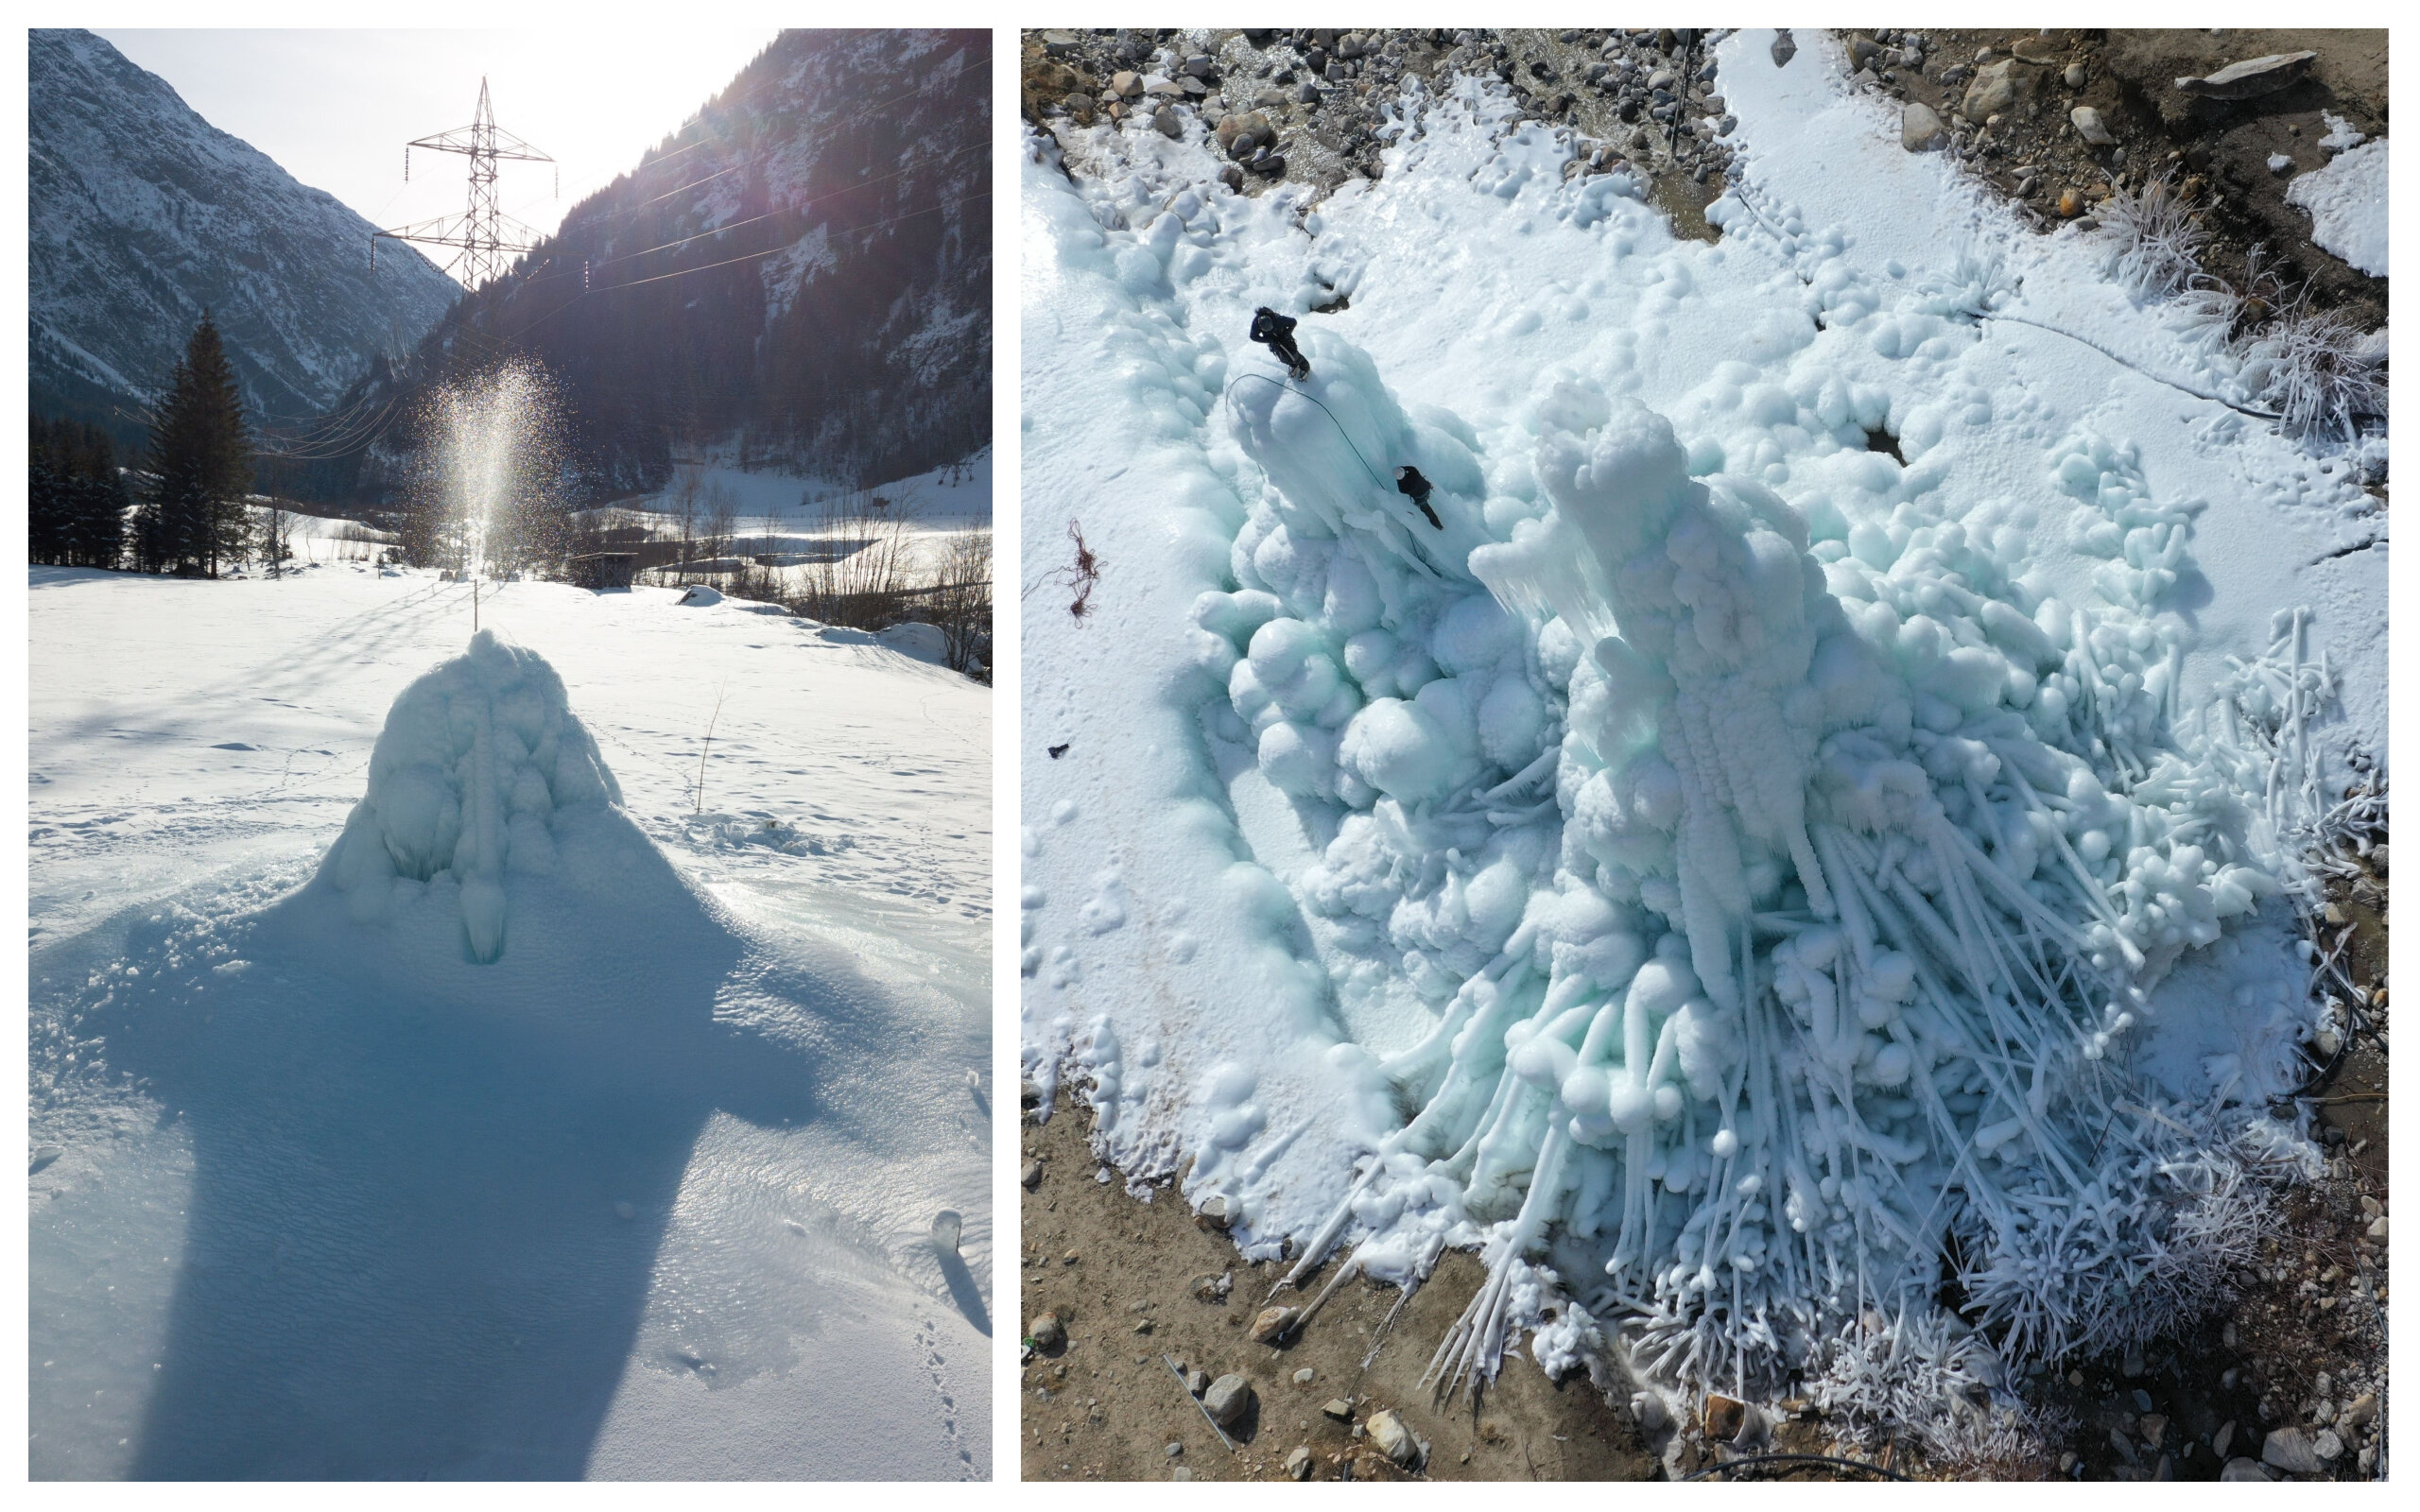
\includegraphics[width=12 cm]{Figures/Figure_2.jpg}
	\end{center}
	\caption{The Swiss and Indian AIR on March 3 and January 9, 2021 respectively. Picture credits: Daniel Buerki (left)
		and Thinles Norboo (right)}
	\label{fig:2AIR}
\end{figure}

The Gangles site (34.22 $\degree$N, 77.61 $\degree$E) is located around 20 km north of Leh city in the Ladakh
region, lying at 4025 $m$ a.s.l.. Because of the rain shadow effect of the Himalayan Range, mean annual
precipitation in Leh totals less than 100 mm, and there is high interannual variability. Whereas the average
summer rainfall between July and September reaches 37.5 mm, the average winter precipitation between January and
March amounts to 27.3 mm and falls almost entirely as snow . The mean annual temperature is $5.6 \, \degree C$,
and the thermal range is characterized by high seasonal variation. During January, the coldest month, the mean
temperature drops to $-7.2 \, \degree C$. During August—the warmest month—the mean temperature rises to $17.5 \,
	\degree C$ \citep{Nusser_2012}. AIR were constructed here as part of the Icestupa Competition  by the Himalayan
Institute of Alternatives, Ladakh (HIAL). The fountain height of the AIR varied between 5 to 9\,$m$.

\subsection{Meteorological data}

Air temperature, relative humidity, wind speed, pressure, longwave, shortwave direct and diffuse radiation are
required to calculate the surface energy balance of an AIR.

For the CH site, the primary weather data source was a Meteoswiss AWS located 184 m away. In addition, we used
ERA5 reanalysis dataset \citep{era5} for filling data gaps and adding data that were not measured directly.  The
ERA5 reanalysis dataset has a good correlation with sites in Switzerland \citep{Scherrer_2020}. The ERA5 grid
point chosen (46.64 $\degree$N, 8.25 $\degree$E) for the Swiss site was around 3.6 km away from the actual site.
ERA5 variables (except incoming shortwave and longwave radiation) were fitted with the meteoswiss dataset via
linear regressions. The zero wind speed values recorded by the Meteoswiss AWS whenever snow accumulated on the
ultrasonic wind sensor were replaced using the ERA5 dataset.

For the IN site, three different weather data sources were used to log all the weather parameters required for
the model. A temperature and humidity logger was placed adjacent to the AIR on a mast. Wind speed and pressure
data was logged via a campbell weather station located 440 m away. Shortwave radiation data was derived from
another campbell weather station located 15 km away. Unfortunately, precipitation was not logged. Since winter
precipitation in Ladakh is less than 30 mm \citep{Nusser_2012}, we can safely assume negligible precipitation
and mostly clear skies. So the diffuse fraction of the global shortwave radiation was also negligible .

\begin{table}
	\centering
	\caption{ Summary of the weather and fountain observations}
	\label{tab:Observations}
	\begin{tabular}{@{}|lllllll|@{}}
		\toprule
		\textbf{}              & \textbf{Name}               & \textbf{Symbol} & \textbf{IN21} &
		\textbf{CH21}          & \textbf{CH20}               & \textbf{Units}                                                              \\ \midrule
		\multicolumn{1}{|l|}{\multirow{9}{*}{\rotatebox[origin=c]{90}{Weather}}}
		                       & Air temperature             & $T_a    $       & $0 \pm 7$     & $2 \pm 6$    & $2
		\pm 4$                 & $\degree C$                                                                                               \\
		\multicolumn{1}{|l|}{} & Relative humidity           & $RH     $       & $35 \pm 20$   & $79 \pm 18$  & $77
		\pm 17$                & \%                                                                                                        \\
		\multicolumn{1}{|l|}{} & Wind speed                  & $v_a        $   & $3 \pm 1$     & $2 \pm 2$    &
		$2 \pm 2$              & $m/s$                                                                                                     \\
		\multicolumn{1}{|l|}{} & Direct Shortwave            & $SW_{direct} $  & $246 \pm 333$ & $80 \pm 156$
		                       & $80 \pm 150$                & $W\,m^{-2}$                                                                 \\
		\multicolumn{1}{|l|}{} & Diffuse Shortwave           & $SW_{diffuse}$  & $0 \pm 0$     & $58 \pm 87$  & $51 \pm 74$  & $W\,m^{-2}$ \\
		\multicolumn{1}{|l|}{} & Incoming Longwave Radiation & $LW_{in}$       & $194 \pm 31$  & $239 \pm 35$ & $236 \pm 34$ & $W\,m^{-2}$ \\
		\multicolumn{1}{|l|}{} & Hourly Precipitation        & $ppt        $   & $0 \pm 0$     & $139 \pm
		457$                   & $95 \pm 404$                & $mm$                                                                        \\
		\multicolumn{1}{|l|}{} & Pressure                    & $p_a         $  & $623 \pm 3$   & $794 \pm 9$  &
		$798 \pm7$             & $hPa$                                                                                                     \\
		\multicolumn{1}{|l|}{} & Observation Duration        & $h_{total} $    & 3673          & 4003
		                       & 1844                        & $hours$                                                                     \\\bottomrule
		\multicolumn{1}{|l|}{\multirow{4}{*}{\rotatebox[origin=c]{90}{Fountain}}}
		                       & Mean discharge              & $d_F     $      & $60$          & $7.5$        &
		$7.5$                  & $l/min$                                                                                                   \\
		\multicolumn{1}{|l|}{} & Runtime                     & $h_F $          & 829           & 2155
		                       & 1553                        & $hours$                                                                     \\
		\multicolumn{1}{|l|}{} & Spray radius                & $r_{F}$         & 10.8          & 6.9
		                       & 7.7                         & $m$                                                                         \\
		\multicolumn{1}{|l|}{} & Water temperature           & $T_{F}$         & 1             & 3
		                       & 3                           & $\degree C$                                                                 \\\midrule
	\end{tabular}
\end{table}


\subsection{Fountain observations}

We define the fountain used through four attributes, namely its spray radius, mean discharge quantity, discharge
runtime and water temperature as shown in Table \ref{tab:Observations}. Continuous measurement of the discharge
rate was unsuccessful in all the sites. Instead the discharge duration was first determined and then the
available discharge measurement was used to determine the average discharge quantity $d_F$ during these periods.
The spray radius $r_F$ was estimated from the mean AIR circumference measured in the drone flights during the
fountain runtime.

The Swiss fountain was never switched off so the discharge duration was extrapolated from just one fountain on
and off event each.

Even though the Indian fountain was never manually switched off, there were many pipeline freezing events that
interrupted the discharge duration. Discharge rate was extrapolated to be the mean discharge $d_F$ except during
these pipeline freezing events.

\subsection{Uncrewed Aerial Vehicle surveys}

Several uncrewed aerial vehicle (UAV) surveys were conducted in the Swiss and Indian sites. The DEM generated
through these flights were analysed to obtain the radius, area and volume of the ice structure.  The first drone
flight was used to set the dome volume ($V_{dome}$) for model initialisation. Since the Indian AIR was built on
top of another ice structure ( see Fig. \ref{fig:2AIR} ), it had a much higher dome volume compared to the other
AIRs.  The number of UAV flights available for the calibration and validation process for the IN21, CH21 and
CH20 AIR were 6, 8 and 2 respectively.  The details of these flights and the methodology used to produce the
corresponding outputs are explained in Appendix \ref{sec:uav} .

\section{Model setup}

A bulk energy and mass balance model is used to calculate the amounts of ice, meltwater, water vapour and runoff
water of the AIR every hour. This model consists of four modules which estimates the AIR a) geometric evolution,
b) energy balance, c) surface temperature, d) mass balance and e) parameter sensitivity.

\begin{figure}
	\begin{center}
		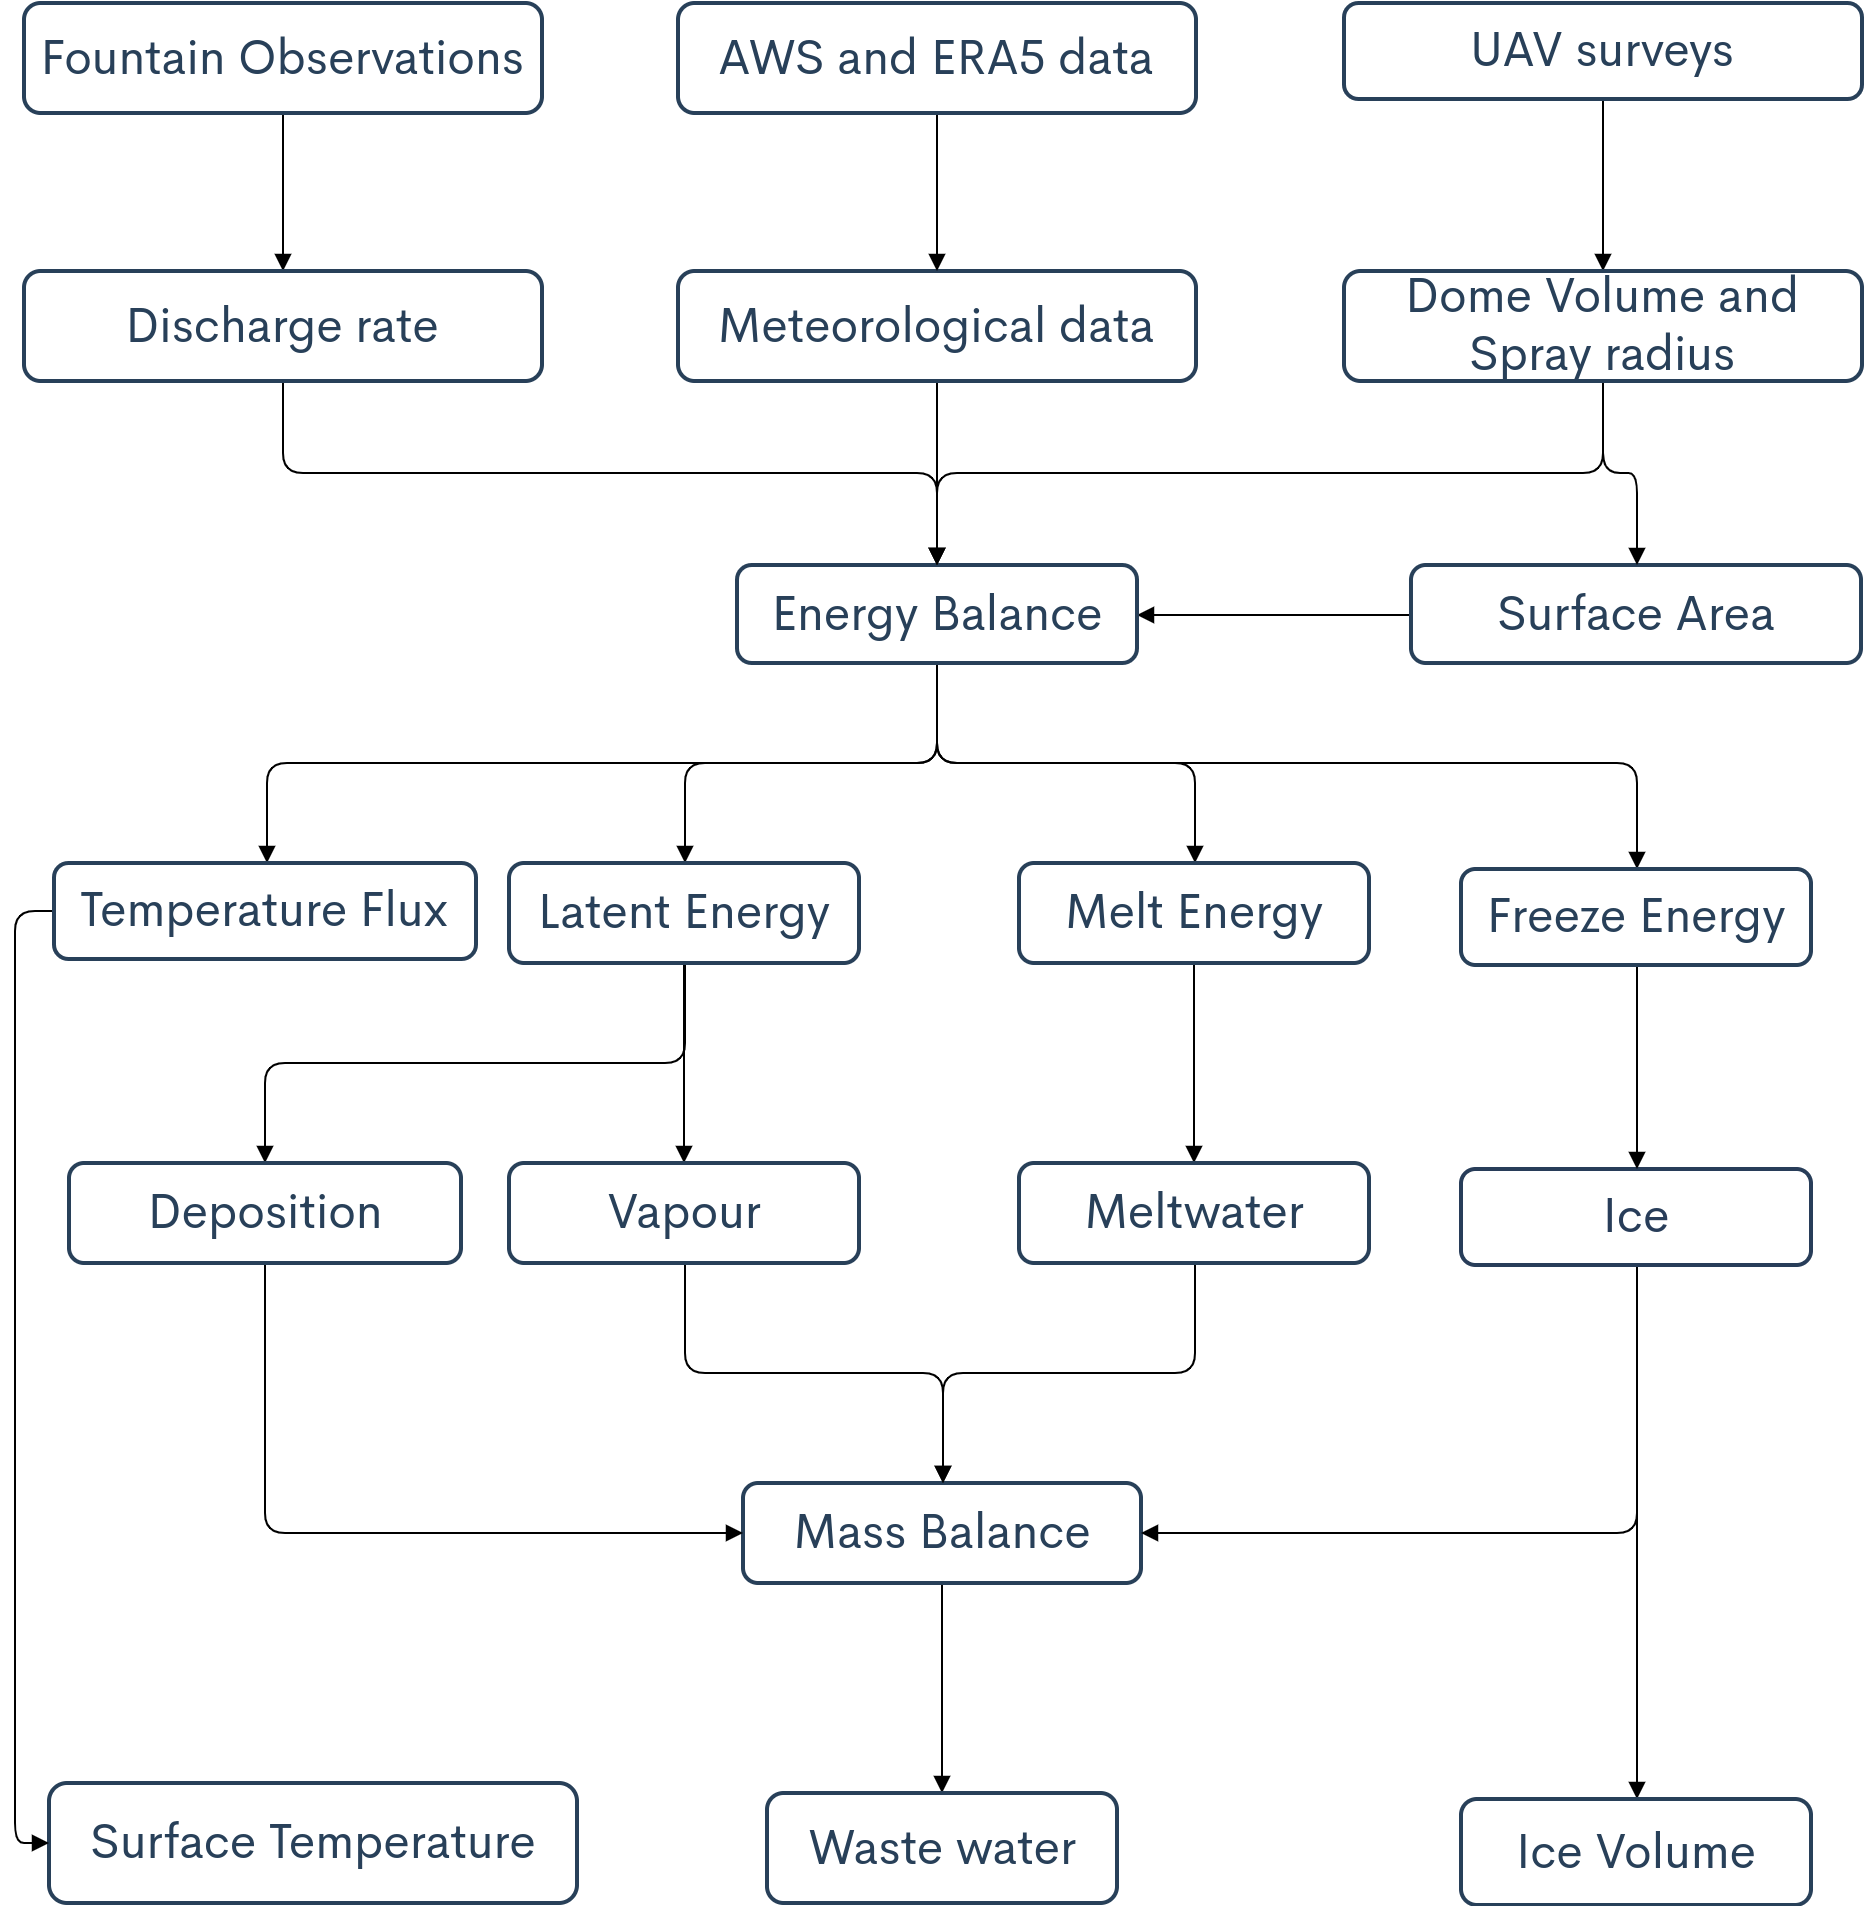
\includegraphics[width=12 cm]{Figures/model_schematic.png}
	\end{center}
	\caption{Model schematic showing the algorithm used in the model at every time step. }
	\label{fig:schema}
\end{figure}

\subsection{Geometric evolution}

Radius $r_{ice}^i$ and height $h_{ice}^i$ define the dimensions of the AIR assuming its geometry to be a cone.
The surface area $A^i$ and volume $V^i$ are:

\begin{equation} A = A_{corr} \cdot \pi \cdot r_{ice} \cdot \sqrt{{r_{ice}}^2 + {h_{ice}}^ 2} \label{eqn:A} \end{equation}

\begin{equation} V = \pi/3 \cdot {r_{ice}}^2 \cdot h_{ice} \label{eqn:V} \end{equation}

where $A_{corr}$ is a correction factor with values between 1 and 2 that accounts for the deviation in AIR
surface area from that of the modelled conical surface. We do not specify the time step superscript $i$ of the
shape variables $A$, $V$, $r_{ice}$ and $h_{ice}$. Henceforth, the equations used, display model time step
superscript $i$ only if it is different from the current time step.


With the mass of the AIR $M_{ice}$, its current volume can also be expressed as:

\begin{equation} V =\frac{M_{ice}} {\rho_{ice}} \label{eqn:V1} \end{equation}

where $\rho_{ice}$ is the density of ice (917 $kg\, m^{-3}$).


The influence of the AIR fountain is parameterised by the fountain water temperature $T_{F}$ and its spray
radius $r_F$.  The initial radius of the AIR is assumed to be $r_F$. The initial height $h_0$ depends on the
dome volume $V_{dome}$ used to construct the AIR as follows:

\begin{equation}
	h_{0} =  \Delta x + \frac{3 \cdot V_{dome}}{\pi r_F^2 }
	\label{eqn:h0}
\end{equation}

where $\Delta x$ is the surface layer thickness (defined in Section \ref{sec:energy})

During subsequent time steps, the dimensions of the AIR evolve assuming a uniform ice formation and decay across
its surface area with an invariant slope $s_{cone} = \frac{h_{ice}}{r_{ice}}$ .  During these time steps, the
volume is parameterised using Eqn. \ref{eqn:V} as:

\begin{equation} V = \frac{\pi \cdot {r_{ice}}^3
		\cdot s_{cone}}{3} \label{eqn:V2} \end{equation}

However, the Icestupa cannot outgrow the maximum range of the water droplets ($(r_{ice})_{max} = r_{F}$).
Combining Eqns. \ref{eqn:V},  \ref{eqn:V1}, \ref{eqn:h0} and \ref{eqn:V2}, the geometric evolution of the
Icestupa at each time step $i$ can be determined by considering the following rules:

\begin{equation} (r_{ice},\, h_{ice}) = \left\{ \begin{array}{ll} (r_F ,\, h_0)                                                                        & \textit{ if } i=0 \\
             (r_{ice}^{i-1},\, \frac{3 \cdot M_{ice}}{\pi \cdot \rho_{ice} \cdot {(r_{ice}^{i-1})}^2}) & \textit{ if }
             r_{ice}^{i-1} \geq r_{F} \textit{ and } \Delta M_{ice} > 0                                                    \\ (\frac{3 \cdot M_{ice}}{\pi \cdot \rho_{ice} \cdot s_{cone}})^{1/3} \cdot (1,\,  s_{cone}) &
             otherwise\end{array} \right.  \label{eqn:A2} \end{equation}

where $\Delta M_{ice} = M_{ice}^{i-1} - M_{ice}^{i-2}$

\begin{figure}
	\begin{center}
		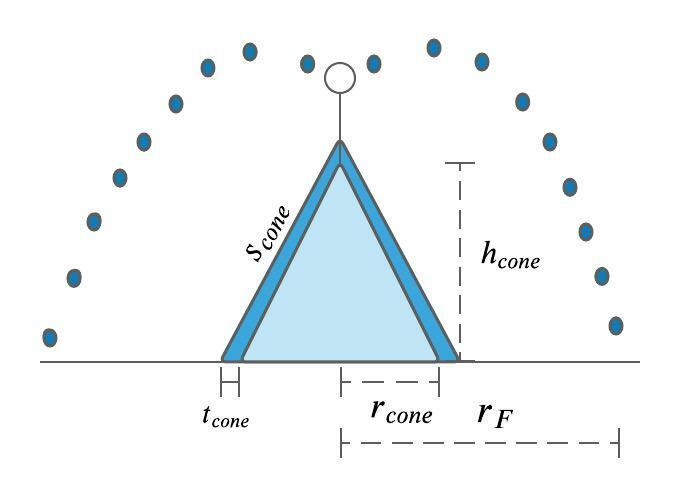
\includegraphics[width=10
			cm]{Figures/shape_parameters.jpeg}
	\end{center}
	\caption{Shape variables and fountain constants of the AIR. $r_{ice}$ is
		the radius, $h_{ice}$ is the height and $s_{cone}$ is the slope of the ice cone. $r_F$ is the spray radius, $h_F$ is the
		height and $T_F$ is the water temperature of the fountain.}
	\label{fig:shape}
\end{figure}

\subsection{Energy Balance} \label{sec:energy}

The energy balance equation (e.g. \cite{Hock_2005}) for the AIR is formulated as follows:

\begin{equation} q_{surf} = q_{SW} + q_{LW} + q_{L} + q_{S} + q_{F} + q_{G}\label{eqn:EB} \end{equation}

where $q_{surf}$ is the surface energy flux in [$W\,m^{-2}$]; $q_{SW}$ is the net shortwave radiation; $q_{LW}$
is the net longwave radiation; $q_{L}$ and $q_{S}$ are the turbulent latent and sensible heat fluxes. $q_{F}$
represents the heat exchange of the fountain water droplets with the AIR ice surface. $q_{G}$ represents ground
heat flux between the AIR surface and its interior. Energy transferred in the direction of the ice surface is
always denoted as positive and away as negative.

Equation \ref{eqn:EB} is usually referred to as the energy budget for “the surface”, but practically it must
apply to a surface layer of ice with a finite thickness $\Delta x$. The energy flux acts upon the AIR surface
layer, which has an upper and a lower boundary defined by the atmosphere and the ice body of the AIR,
respectively. The parameter selection for $\Delta x$ is based on the following two arguments: (a) the ice
thickness $\Delta x$ should be small enough to represent the surface temperature variations every model time
step $\Delta t$ and (b) $\Delta x$ should be large enough for these temperature variations to not reach the
bottom of the surface layer. A sensitivity analysis was later performed to understand the influence of this
factor and decide its value. Here, we define the surface temperature $T_{ice}$ to be the modelled average
temperature of the Icestupa surface layer and the energy flux $q_{surf}$ is assumed to act uniformly across the
Icestupa area $A$.

\subsubsection{Net Shortwave Radiation \texorpdfstring{$q_{SW}$}{Lg}}

The net shortwave radiation $q_{SW}$ is computed as follows:

\begin{equation} q_{SW} = (1- \alpha)\cdot (SW_{direct} \cdot f_{cone} + SW_{diffuse}) \label{eqn:SW} \end{equation}

where $SW_{direct}$ and $SW_{diffuse}$ are the ERA5 direct and diffuse shortwave radiation, $\alpha$ is the
modelled albedo and $f_{cone}$ is the area fraction of the ice structure exposed to the direct shortwave
radiation.

The albedo varies depending on the water source that formed the current AIR surface layer. During the fountain
runtime, the albedo assumes a constant value corresponding to ice albedo. However, after the fountain is
switched off, the albedo can reset to snow albedo during snowfall events and then decay back to ice albedo. We
use the scheme described in \cite{OerlemansKnap_1998} to model this process. The scheme records the decay of
albedo with time after fresh snow is deposited on the surface. $\delta t$ records the number of time steps after
the last snowfall event. After snowfall, albedo changes over a time step, $\delta t$ , as

\begin{equation} \alpha=\alpha_{ice}+(\alpha_{snow}-\alpha_{ice}) \cdot e^{(-\delta t)/\tau} \label{eqn:a}
\end{equation}

where $\alpha_{ice}$ is the bare ice albedo value (0.25), $\alpha_{snow}$ is the snow ice albedo value (0.85)
and $\tau$ is a decay rate (16 $days$), which determines how fast the albedo of the ageing snow reaches this
value.

The area fraction $f_{cone}$ of the ice structure exposed to the direct shortwave radiation depends on the shape
considered. Using the solar elevation angle $\theta_{sun}$, the solar beam can be considered to have a vertical
component, impinging on the horizontal surface (semicircular base of the AIR), and a horizontal component
impinging on the vertical cross section (a triangle). The solar elevation angle $\theta_{sun}$ used is modelled
using the parametrisation proposed by \cite{Woolf_1968}. Accordingly, $f_{cone}$ is determined as follows:

\begin{equation}
	\begin{split}
		f_{cone}& =\frac{(0.5 \cdot r_{ice} \cdot h_{ice}) \cdot cos \theta_{sun} +(\pi \cdot
			{r_{ice}}^2/2) \cdot sin \theta_{sun} }{\pi \cdot r_{ice} \cdot ({r_{ice}}^2+{h_{ice}}^2)^{1/2}}\\
	\end{split}
	\label{eqn:f_{cone}}
\end{equation}

The diffuse shortwave radiation is assumed to impact the conical AIR surface uniformly.

\subsubsection{Net Longwave Radiation \texorpdfstring{$q_{LW}$}{Lg}}

The net longwave radiation $q_{LW}$ is determined as follows:

\begin{equation}
	q_{LW}= LW_{in}-\sigma \cdot \epsilon_{ice} \cdot {(T_{ice}+ 273.15)}^4
	\label{eqn:LW}
\end{equation}

where $T_{ice}$ is the modelled surface temperature, both temperatures are given in [$\degree C$],
$\sigma=5.67\cdot10^{-8}\,Jm^{-2}s^{-1}K^{-4}$ is the Stefan-Boltzmann constant, $LW_{in}$ denotes the incoming
longwave radiation and $\epsilon_{ice}$ is the corresponding emissivity value for the Icestupa surface (0.97).

The incoming longwave radiation $LW_{in}$for the Indian site, where no direct measurements were available, is
determined as follows:

\begin{equation}
	LW_{in}=\sigma \cdot (\epsilon_a \cdot {(T_a+ 273.15)}^4)
	\label{eqn:LWin}
\end{equation}

here $T_a$ represents the measured air temperature and $\epsilon_a$ denotes the atmospheric emissivity. We
approximate atmospheric emissivity $\epsilon_a$ using the equation suggested by \cite{Brutsaert_1982},
considering air temperature and vapor pressure (Eqn.  \ref{eqn:atm_e}). The vapor pressures over air and ice was
obtained using Eqn. \ref{eqn:vp}.  The expression defined in \cite{Brutsaert_1975} for clear skies (first term
in equation \ref{eqn:atm_e}) is extended with the correction for cloudy skies after \cite{Brutsaert_1982} as
follows:

\begin{equation}
	\epsilon_a=1.24 \cdot (\frac{p_{v,a}}{(T_a+273.15)})^{1/7}\cdot(1+0.22\cdot{c}^2) \label{eqn:atm_e}
\end{equation}

with a cloudiness index $c$, ranging from 0 for clear skies to 1 for complete overcast skies. For the Indian
site, we assume cloudiness to be negligible.

\subsubsection{Turbulent fluxes}

The turbulent sensible $q_{S}$ and latent heat $q_{L}$ fluxes are computed with the following expressions
proposed by \cite{Garratt_1992}:

\begin{equation}
	q_{S}=\mu_{cone}\cdot c_{a} \cdot \rho_{a} \cdot p_{a}/p_{0,a} \cdot \frac{\kappa^2 \cdot v_a \cdot
		(T_a-T_{ice})}{{(\ln{\frac{h_{AWS}}{z_{0}}})}^2}
	\label{eqn:qs}
\end{equation}

\begin{equation}
	q_{L}=\mu_{cone}\cdot 0.623 \cdot L_s \cdot \rho_{a}/p_{0,a} \cdot \frac{\kappa^2 \cdot
	v_a(p_{v,a}-p_{v,ice})}{{(\ln{\frac{h_{AWS}}{z_{0}}})}^2}
\end{equation}

where $h_{AWS}$ is the measurement height above the ground surface of the AWS (around $2\,m$ for all sites),
$v_a$ is the wind speed in [$m\,s^{-1}$], $c_a$ is the specific heat of air at constant pressure (1010 J
$kg^{-1} K^{-1}$), $\rho_{a}$ is the air density at standard sea level (1.29 $kg m^{-3}$), $p_{0,a}$ is the air
pressure at standard sea level (1013 $hPa$), $\kappa$ is the von Karman constant (0.4), $z_{0}$ is the surface
roughness (5 $mm$) and $L_s$ is the heat of sublimation (2848 $kJ\,kg^{-1}$).  The vapor pressures over air
($p_{v,a}$) and ice ($p_{v,ice}$) was obtained using the formulation given in \cite{WMO_2018} and
\cite{huang_2018} respectively  :

\begin{equation}
	\begin{split}
		p_{v,a}&=6.107 \cdot 10^{(7.5 \cdot T_a / (T_a + 237.3))} \cdot \frac{RH}{100}\\
		p_{v,ice}&=e^{(43.494 - \frac{6545.8}{T_{ice} + 278})}/(T_{ice} + 868)^2
	\end{split} \label{eqn:vp}
\end{equation}

where $p_{a}$ is the measured air pressure in [$hPa$].

The dimensionless parameter $\mu_{cone}$ is an exposure parameter that deals with the fact that AIR has a rough
appearance and forms an obstacle to the wind regime. This factor accounts for the larger turbulent fluxes due to
the roughness of the surface \citep{Oerlemans_2021}, and is a function of the AIR slope as follows:

\begin{equation}
	\mu_{cone} = 1 + \frac{s_{cone}}{2}
\end{equation}

A possible source of error is the fact that wind measurements from the horizontal plane at the AWS are used,
which might be different from those on a slope. However, without detailed datasets from the AIR surface, we
retain this assumption.

\subsubsection{Fountain discharge heat flux \texorpdfstring{$q_{F}$}{Lg} }

The fountain water temperature $T_F$ is assumed to cool to 0 $\degree C$. Thus, the heat flux caused by this
process is:

\begin{equation}
	q_{F} = \frac{ \Delta M_F \cdot c_{water} \cdot T_F}{\Delta t \cdot A}
	\label{eqn:qF}
\end{equation}

with $c_{water}$ as the specific heat of water.

\subsubsection{Bulk Icestupa heat flux \texorpdfstring{$q_{G}$}{Lg}} \label{sec:Bulkflux}

The bulk Icestupa heat flux $q_{G}$ corresponds to the ground heat flux in normal soils and is caused by the
temperature gradient between the surface layer ($T_{ice}$) and the ice body ($T_{bulk}$). It is expressed by
using the heat conduction equation as follows:

\begin{equation} q_{G} = k_{ice} \cdot (T_{bulk}-T_{ice}^{i-1})/l_{ice} \label{eqn:qG}    \end{equation}

where $k_{ice}$ is the thermal conductivity of ice (2.123 $W\, m^{-1}\,K^{-1}$) , $T_{bulk}$ is the mean
temperature of the ice body within the Icestupa and $l_{ice}$ is the average distance of any point in the
surface to any other point in the ice body. $T_{bulk}$ is initialised as 0 $\degree C$ and later determined from
Eqn. \ref{eqn:qG} as follows:

\begin{equation} T_{bulk}^{i+1} = T_{bulk} - (q_{G} \cdot A \cdot \Delta t)/(M_{ice} \cdot c_{ice}) \end{equation}

Since AIRs typically have conical shapes with $r_{ice} > h_{ice}$, we assume that the center of mass of the ice
body is near the base of the fountain. Thus, the distance of every point in the AIR surface layer from the ice
body's center of mass is between $h_{ice}$ and $r_{ice}$. We calculate $q_{G}$ assuming $l_{ice} = (r_{ice} +
	h_{ice})/2$.

\subsection{Surface temperature}

The available energy $q_{surf}$ can act on the surface of the AIR to a) change its temperature, b) melt ice or
c) freeze ice.

So Eqn. \ref{eqn:EB} can be rewritten as: \begin{equation} q_{surf} = q_{freeze/melt} + q_{T} \end{equation}
where $q_{T}$, $q_{freeze}$ and $q_{melt}$ represent energy associated with process (a), (b) and (c)
respectively.

We categorize the model time steps as freezing or melting events to distribute the surface energy flux into
these three components. Freezing events can only occur, if fountain water is available and the surface energy
flux is negative. However, these two conditions are not sufficient as the latent heat energy can only contribute
to temperature fluctuations. Therefore, for preventing latent heat energy from turning a melting event into a
freezing event an additional condition namely, $(q_{surf}-q_{L}) < 0$, is required.

\begin{equation}
	q_{freeze/melt} = \left\{ \begin{array}{ll}
		q_{freeze} & \textit{ if } \Delta M_{F} > 0 \textit{ and } q_{surf} < 0 \textit{ and }(q_{surf}-q_{L}) < 0 \\
		q_{melt}   & \textit{ otherwise}
	\end{array} \right.
\end{equation}

During a freezing event, the AIR surface is assumed to warm to $0 \degree C$. The available energy
$(q_{surf}-q_{L})$ is further augmented due to this change in surface temperature represented by the energy
flux:

$$q_{0} = \frac{\rho_{ice} \cdot \Delta x \cdot c_{ice} \cdot T_{ice}^{i-1}}{\Delta t}$$

The available energy can either be sufficient or insufficient to freeze the fountain water available. If
insufficient, the additional energy further cools down the surface temperature. The surface energy flux
distribution during a freezing event can be represented as:

\begin{equation}
	(q_{freeze}, q_{T}) = \left\{ \begin{array}{ll}
		(q_{surf}-q_{L}+q_{0}, q_{L}-q_{0}) & \textit{ if } \Delta M_{F} \geq -\frac{(q_{surf}-q_{L}+q_{0}) \cdot A \cdot \Delta
		t}{L_f}                                                                                                                  \\
		(\frac{\Delta M_{F} \cdot L_f
		}{A \cdot \Delta t}
		, q_{surf}+\frac{\Delta M_{F} \cdot L_f
		}{A \cdot \Delta t})                & \textit{ if } \Delta M_{F} < -\frac{(q_{surf}-q_{L}+q_0) A \cdot \Delta
		t}{L_f}
	\end{array} \right.
\end{equation}

During a melting event, the surface energy flux ($q_{surf}$) is first used to change the surface temperature to
$T_{temp}$ calculated as:

\begin{equation} T_{temp} =\frac{q_{surf} \cdot \Delta t}{\rho_{ice} \cdot c_{ice} \cdot \Delta x} + T_{ice} \end{equation}

If $T_{temp} > 0 \degree C$, then energy is reallocated from $q_{T}$ to $q_{melt}$ to maintain surface
temperature at melting point. The surface energy flux distribution during a melting event can be represented as:

\begin{equation}
	(q_{melt}, q_{T}) = \left\{ \begin{array}{ll}
		(0, q_{surf})                                                                                                                                                 & \textit{ if } T_{temp} < 0 \\
		(\frac{T_{temp} \cdot \rho_{ice} \cdot c_{ice} \cdot \Delta x}{\Delta t}, q_{surf}-\frac{T_{temp} \cdot \rho_{ice} \cdot c_{ice} \cdot \Delta x}{\Delta t}  ) & \textit{ if } T_{temp} > 0
	\end{array} \right.
\end{equation}


\subsection{Mass Balance}

The mass balance equation for an AIR is represented as:

\begin{equation}
	\frac{\Delta M_{F} + \Delta M_{ppt} + \Delta M_{dep}}{\Delta t} = \frac{\Delta M_{ice} +\Delta M_{water} +
		\Delta M_{sub} + \Delta M_{runoff}}{\Delta t}  \\
	\label{eq:MB}
\end{equation}

where $M_{F}$ is the discharge of the fountain; $M_{ppt}$ is the cumulative precipitation;  $M_{dep}$ is the cumulative
accumulation through water vapour deposition; $M_{ice}$ is the cumulative mass of ice; $M_{water}$ is the cumulative
mass of melt water; $M_{sub}$ represents the cumulative water vapor loss by sublimation and $M_{runoff}$ represents the
fountain discharge runoff that did not interact with the AIR. The LHS of equation \ref{eq:MB} represents the rate of
mass input and the RHS represents the rate of mass output for an AIR.

Precipitation input is calculated as shown in equation \ref{eq:ppt} where $\rho_{w}$ is the density of water (1000
$kg\,m^{-3}$), $ppt$ is the measured precipitation rate in [$m\,s^{-1}$] and $T_{ppt}$ is the temperature threshold
below which precipitation falls as snow. Here, snowfall events were identified using $T_{ppt}$ as $1 \degree C$. Snow
mass input is calculated by assuming a uniform deposition over the entire circular footprint of the AIR.

The latent heat flux is used to estimate either the evaporation and condensation processes or sublimation and deposition
processes as shown in equation \ref{eq:vap}. During time steps at which surface temperature is below 0 $\degree C$ only
sublimation and deposition can occur, but if the surface temperature reaches 0 $\degree C$, evaporation and condensation
can also occur. As the differentiation between evaporation and sublimation (and condensation and deposition) when the
air temperature reaches 0 $\degree C$ is challenging, we assume that negative (positive) latent heat fluxes correspond
only to sublimation (deposition), i.e. no evaporation (condensation) is calculated.

Since we have categorized every time step as a freezing and melting event, we can determine the meltwater and  ice
generated using the associated energy fluxes as shown in equations \ref{eq:mwat} and \ref{eq:mice}. Having calculated
all the other mass components the fountain wastewater generated every time step can be calculated using Eqn.
\ref{eq:MB}.

\begin{subequations}
	\label{equations}
	\begin{align}
		\label{eq:ppt}
		\frac{\Delta M_{ppt}}{\Delta t}                                    & = \left\{ \begin{array}{ll} \pi \cdot {r_{ice}}^2 \cdot
			\rho_{w}\cdot ppt & \textit{ if } T_{a} < T_{ppt} \\ 0 & \textit{ if } T_{a} \geq T_{ppt} \\\end{array} \right.                                      \\
		\label{eq:vap}
		(\frac{\Delta M_{dep}}{\Delta t}, \frac{\Delta M_{sub}}{\Delta t}) & = \left\{ \begin{array}{ll} \frac{q_{L}
			\cdot A}{L_s}\cdot (1,0)  & \textit{ if } q_{L} \geq 0 \\ \frac{q_{L}
			\cdot A}{L_s}\cdot (0,-1) & \textit{ if } q_{L} < 0    \\\end{array} \right.                                      \\
		\label{eq:mwat}
		\frac{\Delta M_{water}}{\Delta t}                                  & = \frac{q_{melt} \cdot A }{L_f}                                                   \\
		\label{eq:mice}
		\frac{\Delta M_{ice}}{\Delta t}                                    & = \frac{q_{freeze}\cdot A }{L_f} + \frac{\Delta M_{ppt}}{\Delta t} + \frac{\Delta
			M_{dep}}{\Delta t}- \frac{\Delta M_{sub}}{\Delta t}- \frac{\Delta M_{melt}}{\Delta t}
	\end{align}
\end{subequations}

We define the freezing rate $M_{freeze}$ and the melting rate $M_{melt}$ as follows:

\begin{equation}
	M_{freeze/melt} = \frac{q_{freeze/melt} \cdot A }{L_f}
	\label{eq:m_freeze/melt}
\end{equation}

To estimate the mass of any component at time step $i$, one can now sum the mass flux estimated above: \begin{equation}
	M_{comp}^i = \sum_{t=0}^{t=i} (\frac{\Delta M_{comp}}{\Delta t})_{t} + M_{comp}^0 \end{equation} where

\begin{equation} M_{comp}^0 = \left\{ \begin{array}{ll} -V_{dome} * \rho_{ice} & \textit{ if } M_{comp}=
             M_{ice}\textit{ or }
             M_{F}                                                 \\ 0 & \textit{ otherwise }\\\end{array} \right. \\
\end{equation}

Considering AIRs as water reservoirs, their net water loss ($NWL$) can be defined as:

\begin{equation} \textit{NWL} = \frac{M_{runoff}+M_{sub}}{(M_F+M_{ppt}+M_{dep})} \cdot 100 \end{equation}

Since this model uses a surface energy balance model commonly applied on glaciers, we define the AIR thickness
balance (TB) analogous to glacier mass balance using its surface normal thickness change with units of $m
	\,w.\,e.$. The thickness balance (TB) for any AIR defined as:

\begin{equation} TB =m_{ice}=\Delta M_{ice}/A \end{equation}

Note that the surface normal thickness is not conserved during the lifetime of the AIR since the surface area
varies unlike that of a glacier but it is conserved for each time step, so Eqn. \ref{eq:MB} can be rewritten as
follows:

\begin{equation}
	m_{F} + m_{ppt} + m_{dep} = m_{ice} +m_{water} + 	m_{sub} + m_{runoff}  \\
	\label{eq:TB}
\end{equation}

\subsection{Sensitivity and uncertainty analysis}

We used a polynomial chaos expansion approach (as in \cite{uncertainpy_2018}; \cite{Xiu_2005}) to evaluate the
model sensitivity and uncertainty. Polynomial chaos expansion are a much more efficient way to obtain similar
results compared to the computationally demanding Monte Carlo methods. This approach approximates the model with a
polynomial (as a surrogate model), on which sensitivity and uncertainty analysis can be performed.  The surrogate
model produced was a polynomial of order 4.

The uncertainty in the model of estimating ice volumes are caused due to two sources, namely, the weather
conditions and the fountain parameters. For the weather parameters, we first fix a range based on literature values
and then perform a global sensitivity analysis (GSA) with the net water loss ($NWL$) as the objective. The
distribution is always treated as uniform and the limits for every parameter are given in Table
\ref{tab:parameters}. The GSA consists of a total ensemble size of 2000 simulations per AIR. The parameter
sensitivity results from the GSA are used as a tool to reduce the number of free parameters in the model by
identifying those parameters, which have only a marginal influence on the model output.

The ranges for the snow albedo were taken from \cite{ZollesMaussion_2019}; ice albedo minimum was taken from
\cite{steiner_2015} and maximum from \cite{ZollesMaussion_2019}; albedo decay rate is assumed to have a minimum
value of 10 days similar to values obtained by \cite{Schmidt_2017} for wet surfaces and a maximum of 22 days from
\cite{OerlemansKnap_1998}; emissivity range from \cite{steiner_2015} and temperature threshold for precipitation
from \cite{Zhou_2010}. The surface area correction factor, $A_{corr}$, quantifies the deviation of the AIR shape
from the conical shape assumed in the model. We assume the range of this deviation to be between 1 to 2. Values for
surface roughness, $z_{0}$, of glacier ice are generally in the range $0.1-5\, mm$ \citep{BrockWillisSharp_2006}.
Since the surface layer thickness, $\Delta x$, for an AIR does not bear resemblance to any parameter in the
glaciological literature, we attribute a wide range of values for it.

The uncertainty associated with fountain parameters listed in Table \ref{tab:Observations} was quantified
separately. Fountain runtime has no uncertainty for the Swiss AIRs because no interruptions were caused during
water distribution. However, significant uncertainty exists for the IN21 AIR , where the interruptions due to
pipeline freezing events happened overnight but this was ignored in this analysis. The choice of $d_F$ for both
sites was just a best guess, based on few observations made by the flowmeter. So we associate this parameter by a
large uncertainty of $\pm \,50\, \%$. For the fountain water temperature, we set a lower and upper bound of $0\,
	\degree C$ and $3\, \degree C$.  It is very unlikely for the fountain water to have been beyond this range
considering winter conditions at all the sites.

Uncertainty also exists in the model input data, particularly for all the radiation measurements ($SW_{direct},
	SW_{diffuse}, LW_{in}$) since they were taken from ERA5 dataset or an AWS away from the construction sites.  But we are
not accounting for uncertainties related to meteorological forcing data in this analysis.

The sensitivity analysis and calibration was carried out for the CH21 and IN21 AIRs and the CH20 AIR was used for
validation of the model.

\begin{table}
	\centering
	\caption{The ranges of the 8 weather parameters used in the sensitivity and uncertainty analysis.}
	\label{tab:parameters}
	\begin{tabular}{@{}llllll@{}}
		\toprule
		\textbf{No.} & \textbf{Name}                       & \textbf{Abbreviation} & \textbf{Min} & \textbf{Max} & \textbf{Unit} \\\midrule
		1            & Ice Emissivity                      & $\epsilon_{ice}$      & 0.95         & 0.99         &               \\
		2            & Ice Albedo                          & $\alpha_{ice}$        & 0.15         & 0.35         &               \\
		3            & Snow Albedo                         & $\alpha_{snow}$       & 0.8          & 0.9          &               \\
		4            & Precipitation Temperature threshold & $T_{ppt}$             & 0            & 2            & $\degree C$   \\
		5            & Albedo Decay Rate                   & $\tau$                & 10           & 22           & $days$        \\
		6            & Surface Roughness                   & $z_0$                 & 1            & 5            & $mm$          \\
		7            & Surface Area correction factor      & $A_{corr}$            & 1            & 2            &               \\
		8            & Surface layer thickness             & $\Delta x$            & 10           & 50           & $mm$          \\\bottomrule
	\end{tabular}
\end{table}

\section{Results}

\subsection{Sensitivity analysis}

The focus of the GSA is not on the absolute sensitivity towards single parameters, but rather to reduce the
dimension of the parameter space. Therefore, the following discussion is limited to two classes: parameters to
which the model is sensitive ($S_{T_{i}} > 0.2$) and non-sensitive ($S_{T_{i}} \leq 0.2$). The threshold of 0.2 was
chosen since most of the parameters were bounded by it. For all the AIRs, just three parameters were sensitive
namely, $z_{0}$, $A_{corr}$ and $\Delta x$. Model simulations were carried out varying all the sensitive parameters
within the ranges defined in Table \ref{tab:parameters}.

Two objectives were chosen namely, ice volume and area, to determine the model performance with respect to these
sensitive parameters. The frequency distribution  of RMSE determined between the UAV observations (see Table
\ref{tab:uav}) and the model outputs among the best 10 \% runs are shown in Fig.\ref{fig:param_hist} for each objective
on each AIR.

\begin{figure}
	\begin{center}
		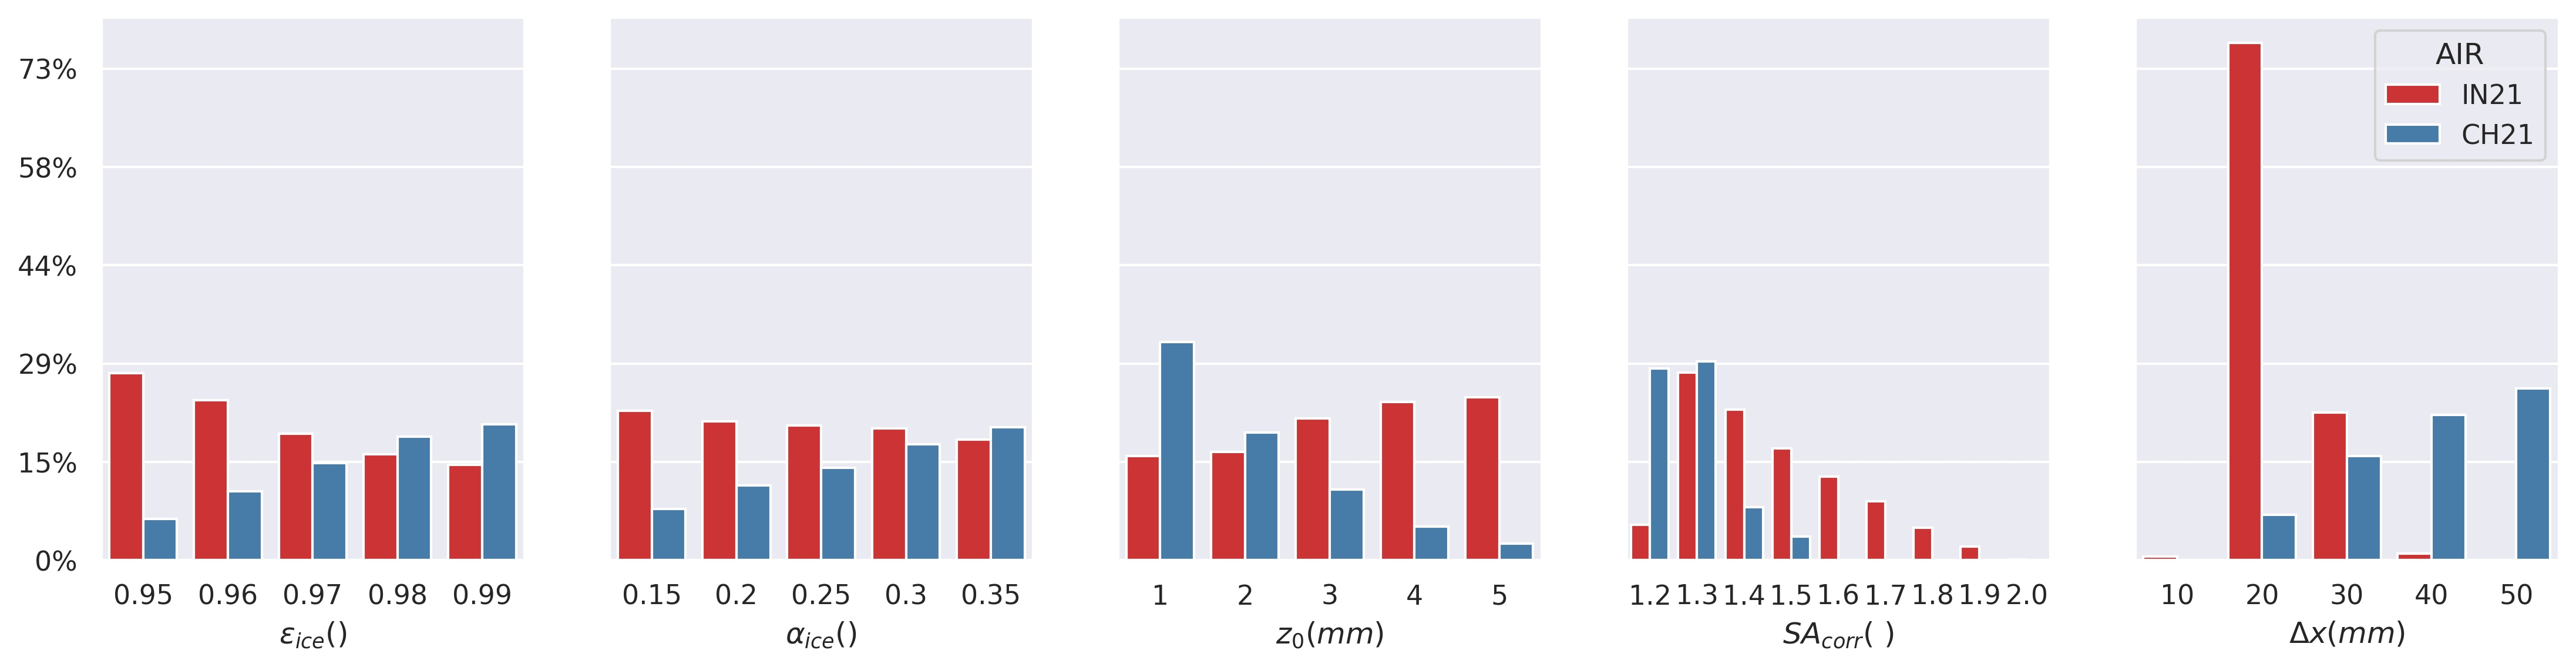
\includegraphics[width=\linewidth]{Figures/param_hist.jpg}
	\end{center}
	\caption{Observed ranges of the sensitive parameters used in the model optimization, shown by
		plotting the frequency distribution of the parameter values for the best 10 \% of the model runs. }
	\label{fig:param_hist}
\end{figure}

\subsection{Calibration}

For model calibration, we choose values of sensitive parameters populating more the 50 \% of the possibilities
among the best 10 \% of the model runs. In total, 495 model runs were required for each of the objective.
For the volume prediction, the RMSE of the best model runs ranged from 26 $m^3$ to 58 $m^3$ for the IN21 and from
10 $m^3$ to 16 $m^3$ for the CH21. For the area prediction, the RMSE of the best model runs ranged from 14 $m^2$ to
53 $m^2$ for the IN21 and from 28 $m^2$ to 40 $m^2$ for the CH21. Note that this calibration process has an
inherent temporal bias due to the choice of when and how many UAV flights were possible in each location. Among
the 5 flights of IN21 AIR used for calibration, most of them were flown around early March when the AIR volume was
near its maximum whereas the CH21 flights were more evenly spaced out in comparison (see Table \ref{tab:uav}).

$A_{corr}$ shows different preferences whereas the other two parameters show similar preference for the two
objectives. We expect the UAV measured surface area of the AIRs to be higher than the modelled cone area due to the
additional surface area caused by its various ice features. Particularly, we expect the IN21 surface area to
deviate significantly from CH21 AIR because its surface area represents the area of two ice cones merged into one
(see Fig.  \ref{fig:2AIR}). This is clearly represented in the disjoint frequency distribution of the area
objective of the CH21 and IN21 AIR. Hence, we calibrate the IN21 area correction factor to 1.5. Since no strong
preference is observed for the CH21 area correction factor, we calibrate it to the median of the values it assumed
in the area objective, namely, 1.2.

The model surface layer thickness was selected based on the two conditions described in Section \ref{sec:energy}.
Since the minimum surface temperature does not go beyond $-30 \, \degree C$ (satisfies (b)) for the smallest
possible thickness of $20\, mm$ (satisfies (a)), we have taken this as the model surface layer thickness.

For the surface roughness, no clear preference is observed for the IN21 AIR, so we calibrated it to the median
value of $3 \, mm$. For the CH21 AIR, it is assigned its preferred value of $1 \, mm$.

\subsection{Weather and fountain uncertainty analysis}

The uncertainty in the ice volume estimates caused by the insensitive model and fountain parameters are shown in
Fig. \ref{fig:results}. The ranges highlighted represent the 90 \% prediction interval of the ice volume estimates.
Weather uncertainty determination required 254 simulations whereas fountain uncertainty determination required 200 simulations.

Weather uncertainty for IN21 is low compared to the other AIRs since precipitation and the associated variation in
albedo was negligible. This is expected since 4 out of the 5 insensitive parameters are part of the albedo module.
The remaining parameter, ice emissivity, caused the most variance in the ice volume estimate among all the
insensitive parameters ($S_{T_{i}} = 0.7$).

Fountain uncertainty for all the AIRs was high showcasing the importance of quantifying the fountain parameters for
a confident ice volume estimation. Among the 3 fountain parameters, ice volume variation was caused predominantly
by the uncertainty in the spray radius ($S_{T_{i}} = 0.8$).

\begin{figure}
	\begin{center}
		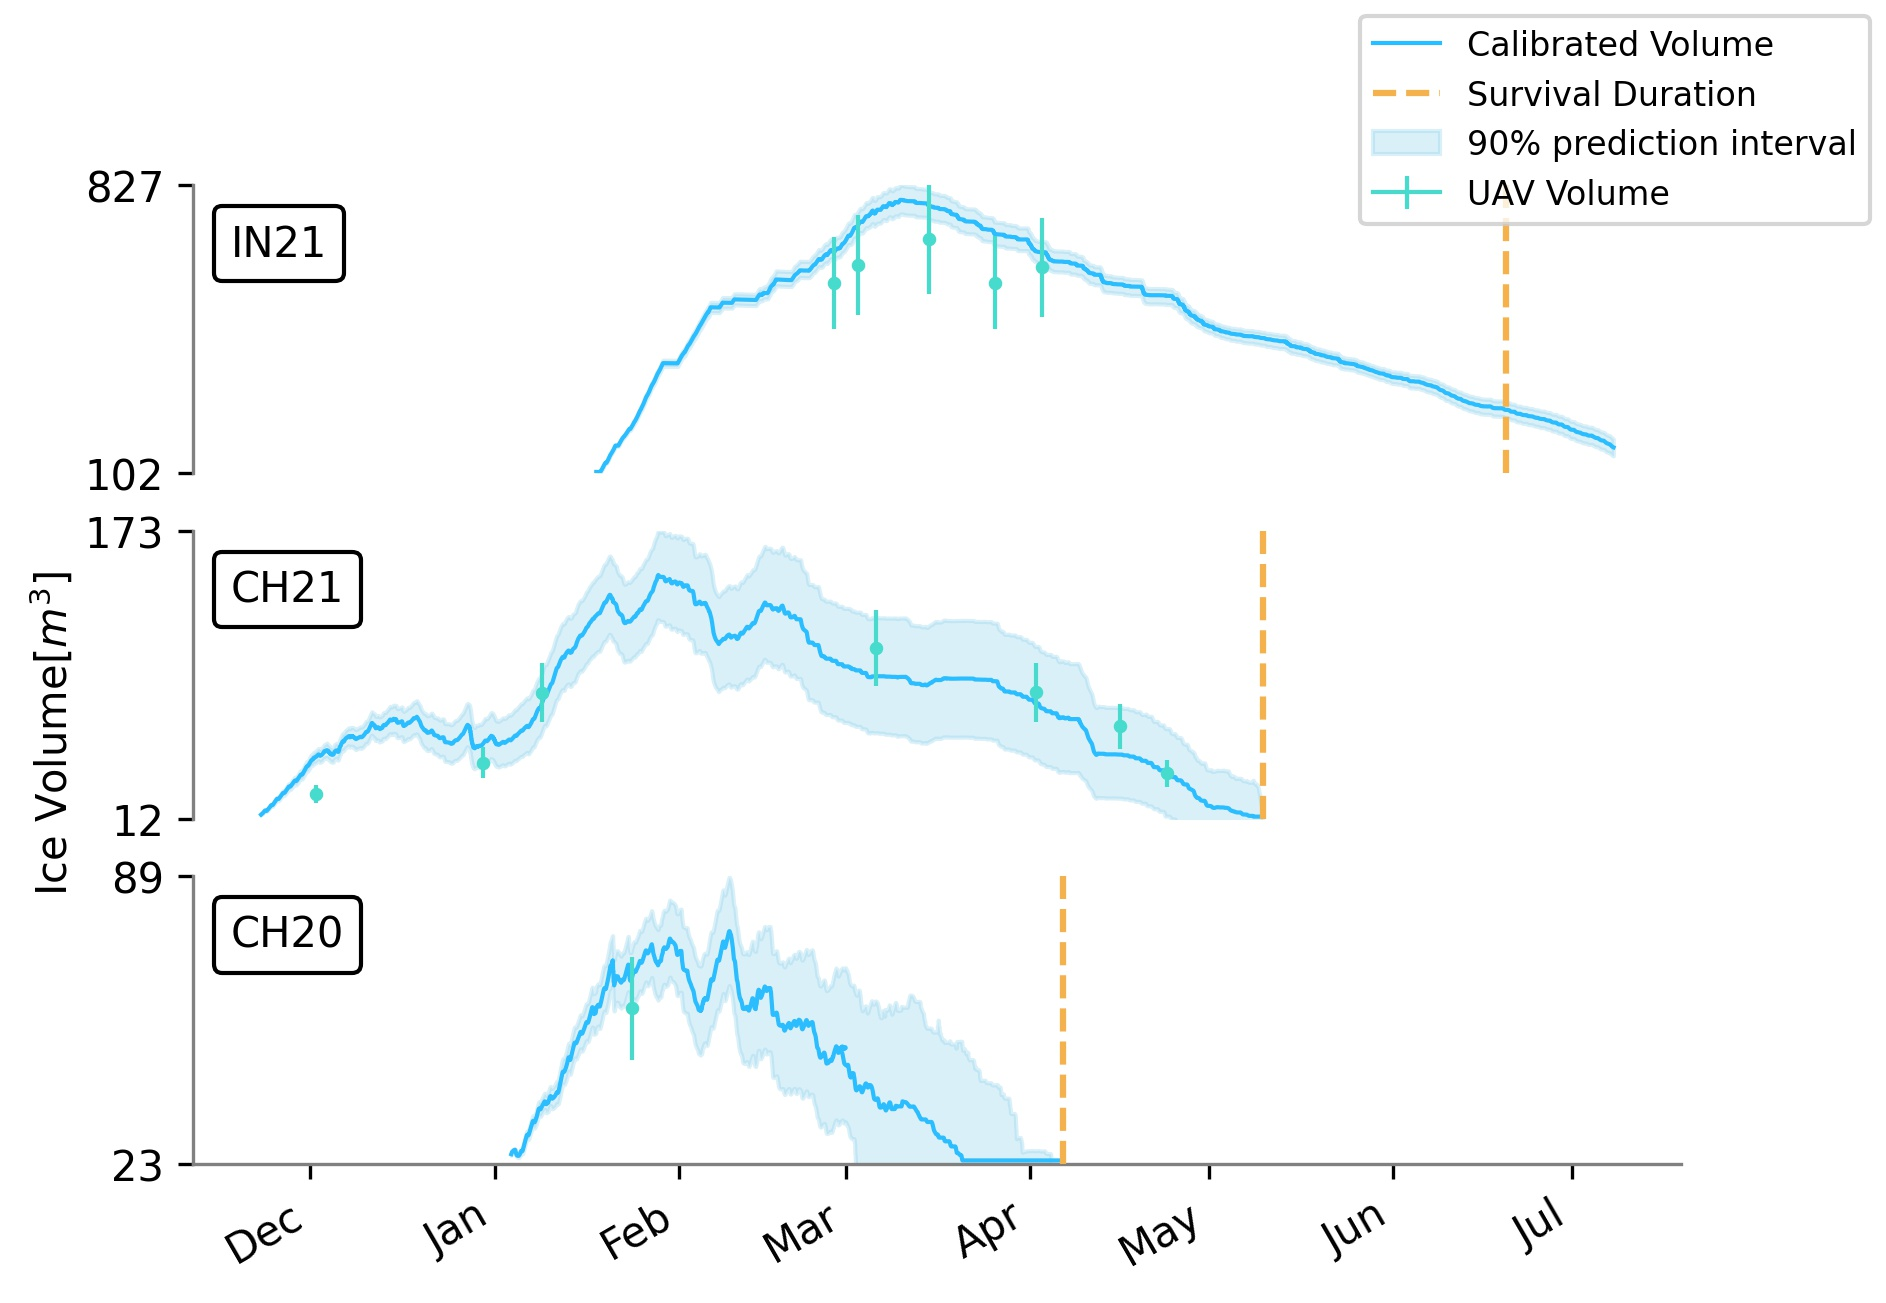
\includegraphics[width=\linewidth]{Figures/icev_results.jpg}
	\end{center}
	\caption{Modelled ice volume during the lifetime of the AIRs (blue curve). The shaded regions (light blue and orange)
		represent the 90\% prediction interval of the AIR ice volume caused by the variation in weather and the fountain parameters.
		The lower bounds of the y-axis represents AIR dome volume. Green points indicate the UAV ice volume observations.
		The violet line represents the observed melt-out date for each AIR.  }

	\label{fig:results}
\end{figure}

\subsection{Validation}

The calibrated model is validated using two datasets, namely, CH20 AIR dataset and the melt-out observations for
each AIR. The melt-out date signifies the time when all the ice has completely disappeared and only the dome volume
remains. Model performance can be judged based on the difference between the model expectation and observation of
melt-out date.  So model performance for the CH21 and CH20 AIRs was -1 day and -16 days, respectively. The negative
sign represents underestimation of the melt-out date. For the IN21 AIR, the determination of the melt-out date was
not possible both through observation and through modelling.  In reality, the IN21 AIR was found to have
disintegrated into several ice blocks on 20th June, 2021.  Model expectation of melt-out date was also not defined
since the AIR never melted completely during the model duration.

There was just one UAV observation of the CH20 AIR Volume (see Table \ref{tab:uav}).  The RMSE of that UAV ice
observation with the modelled volume was just $9 m^3$.

\subsection{AIR ice volume estimates}

The construction decisions responsible for the observed magnitude and variance of the ice volume estimates can
be categorised based on the fountain used and the site location selected. According to Eqn.
\ref{eq:m_freeze/melt}, the freezing/melting rate of the AIRs can be decomposed to the corresponding
freezing/melting energy and the surface area. The construction location chosen determines the freezing/melting
energy flux through its weather and the fountain determines the surface area through its spray radius.

\subsubsection{Location influence}

The influence of location can be further comprehended, if we analyse the daily surface normal thickness change
together with the freezing/melting energy flux. The daily surface normal thickness change is equivalent to the
mass balance terminology used in glaciological literature and is referred as such in the following
analysis. Fig.  \ref{fig:MEB} shows the daily mass and energy balance components calculated with the calibrated
parameters for the first and last 20 days for each AIR. The two time periods selected are characteristic of the
freezing and melting period, respectively. A strong variability is evident between the freezing and melting
periods and between the CH21 and the IN21 AIR.

The magnitudes of the thickness balance components (TBC) in Fig. \ref{fig:MEB} are explained by their corresponding
energy balance component (EBC).  Particularly, ice TBC corresponds to freezing EBC, melt TBC corresponds to melting
EBC available and the net TBC represents the surface EBC available.  Snow deposition is calculated directly from
the precipitation quantity and the sublimation/deposition quantities corresponding to the latent heat EBC
available.  The rest of the EBC components are shown to represent the different physical processes that
contribute to this freezing and melting EBC components.

The mean TB of the Indian location was positive ($1\, mm \,w.e.$) whereas in the Swiss location it was negative
($-3\, mm \,w.e.$). This was because the mean freezing EBC was higher than the melting EBC for the Indian site
whereas this was not the case for the Swiss site as can be seen from Table \ref{tab:Observations}.

\begin{figure}
	\begin{center}
		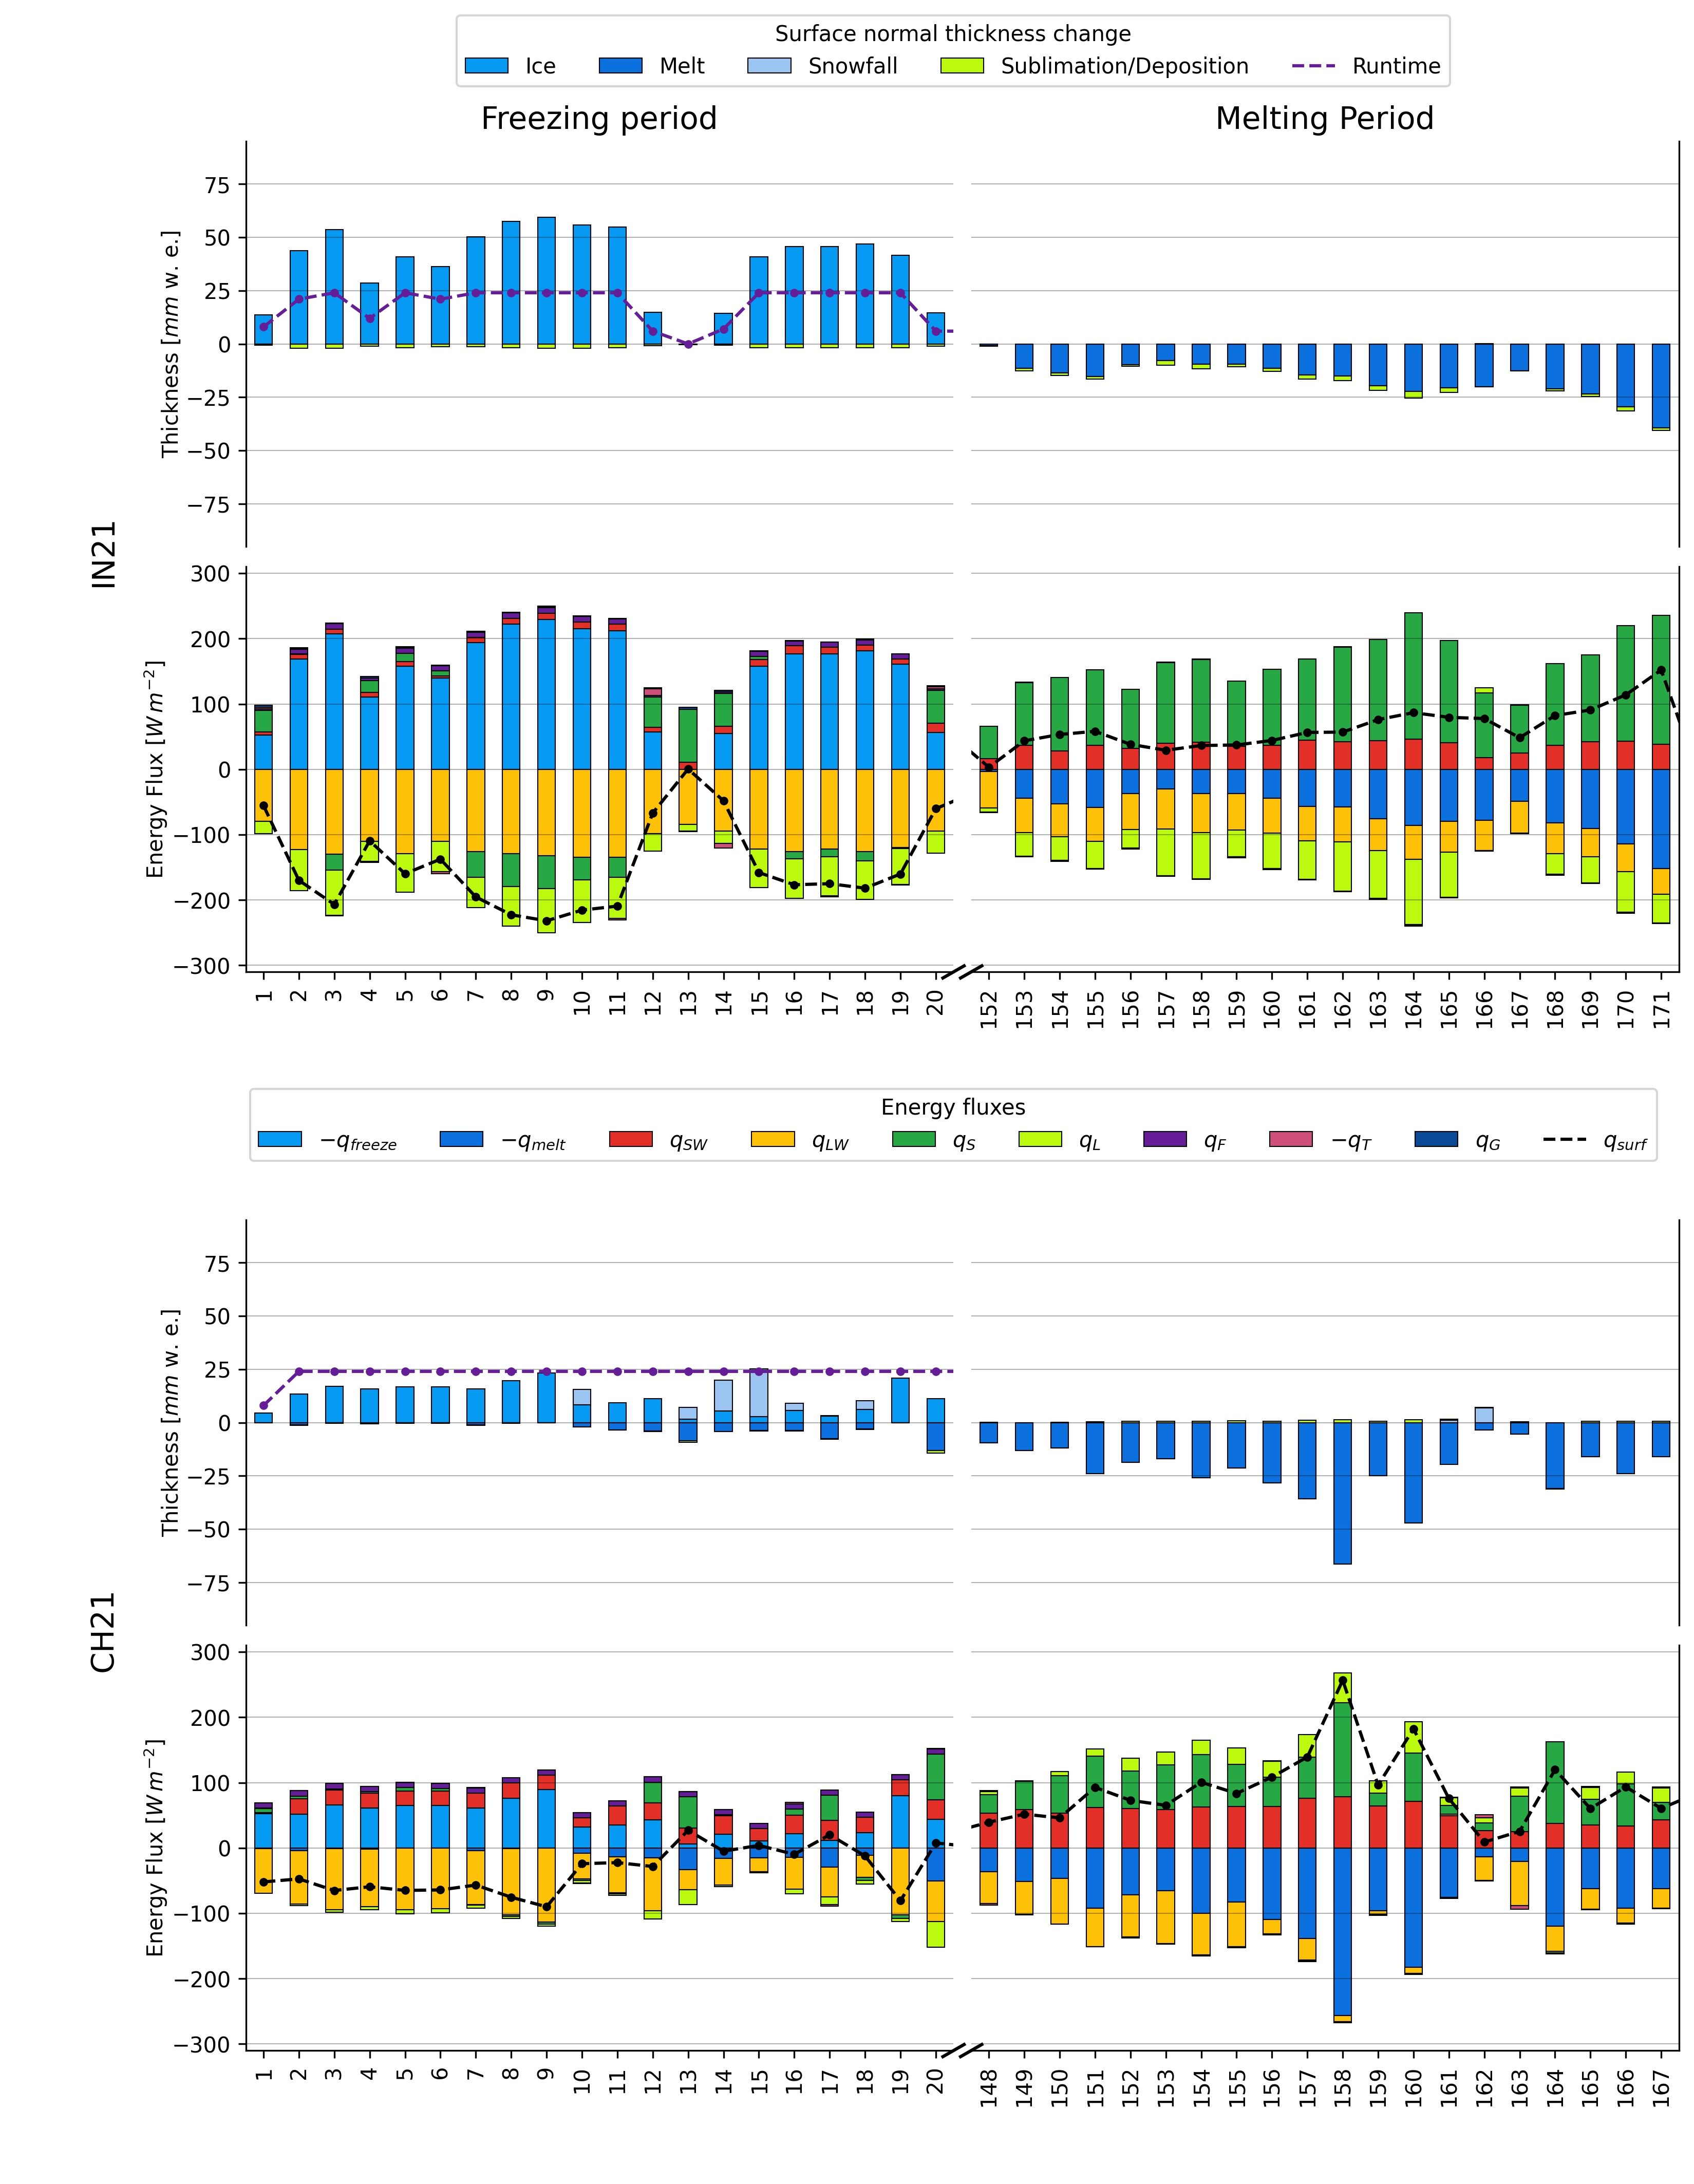
\includegraphics[width=\linewidth]{Figures/mass_energy_bal.jpg} \end{center}
	\caption{Daily averages of mass and energy balance components compared for the Indian and Swiss AIRs during
		the first 20 days of the freezing and the last 20 days of the melting period respectively.  } \label{fig:MEB} \end{figure}

The largest contributor to the freezing EBC was the longwave radiation flux for all the locations.  It also
compensates the shortwave radiation to a large degree during the melting period. The variability of longwave
radiation for the Indian and the Swiss sites was low but the magnitude was much higher for the Indian site. This
is because the  magnitude of incoming longwave radiation was lower for the Indian site due to its low cloudiness
(see Table \ref{tab:Observations}).

The largest contributor to the melting EBC was the sensible heat flux for all the locations. The IN21 AIR melted
gradually but the CH21 AIR melted rapidly on certain days (e.g.  day 140) due to the well-known foehn events
(Reference). These foehn events produced meltwater at the Swiss location sites even during the freezing periods
(e.g.  day 17).

Latent heat plays a very important role in the energy balance. It contributes to both TBC and EBC simultaneously
through deposition/sublimation processes. On first glance, the mass flux shown in Table \ref{tab:Observations}
suggests that sublimation was also a source of water loss but the corresponding energy flux of this process
generated much more ice mass since the heat of vaporization is around nine times higher than the heat of fusion.
The magnitude of the sublimation process was significantly different for both the AIRs. IN21 AIR lost 4 \% of
its mass input to sublimation compared to the 1 \% for the CH21 AIR as the corresponding latent heat fluxes were
an order of magnitude larger (see Table \ref{tab:Observations}). For the IN21 AIR, mass gain due to the
deposition process was negligible compared to the mass loss due to the sublimation process. For the CH21 AIR,
half of the mass lost to sublimation was regained by deposition.  These process differences were primarily
caused by the two fold difference in relative humidity between the sites. This was expected since glaciers near
the IN21 location have been hypothesized to lose a significant amount of mass through sublimation by
\cite{azam_2018}.

Direct shortwave radiation is more than three times higher for the IN21 location due to its higher altitude and
lower latitude. However, there is no significant difference in the net shortwave radiation absorbed by both the
AIRs. The higher diffuse shortwave radiation at the Swiss location is compensating for its lower direct
shortwave radiation (see Table \ref{tab:Observations}). Since the IN21 site has mostly clear days, its diffuse
shortwave radiation was strongly reduced. Moreover, less than half of the AIR surface area was exposed to direct
shortwave radiation flux for both the locations due to the area fraction $f_{cone}$.   Albedo, on the other
hand, only varied for the Swiss location because there was no precipitation for the IN21 site.

\begin{table}
	\centering
	\caption{ Summary of the mass balance, energy balance and AIR characteristics estimated by the model}
	\label{tab:Results}
	\begin{tabular}{@{}|llllll|@{}}
		\toprule
		\textbf{}              & \textbf{Name}                   & \textbf{Symbol} & \textbf{IN21} & \textbf{CH21} &
		\textbf{Units}                                                                                                           \\ \midrule
		\multicolumn{1}{|l|}{\multirow{3}{*}{\rotatebox[origin=c]{90}{Input}}}
		                       & Fountain discharge              & $M_F$           & 2888          & 971           & $tons$      \\
		\multicolumn{1}{|l|}{} & Snowfall                        & $M_{ppt}$       & 0             & 55            & $tons$      \\
		\multicolumn{1}{|l|}{} & Deposition                      & $M_{dep}$       & 12            & 4             & $tons$      \\ \midrule
		\multicolumn{1}{|l|}{\multirow{4}{*}{\rotatebox[origin=c]{90}{Output}}}
		                       & Meltwater                       & $M_{water}$     & 435           & 227           & $tons$      \\
		\multicolumn{1}{|l|}{} & Ice                             & $M_{ice}$       & 148           & 0             & $tons$      \\
		\multicolumn{1}{|l|}{} & Sublimation                     & $M_{sub}$       & 128           & 8             & $tons$      \\
		\multicolumn{1}{|l|}{} & Fountain runoff                 & $M_{runoff}$    & 2287          & 795           & $tons$      \\ \midrule
		\multicolumn{1}{|l|}{\multirow{10}{*}{\rotatebox[origin=c]{90}{Energy flux}}}
		                       & Shortwave radiation             & $q_{SW} $       & $ 26 \pm 43$  & $ 37 \pm 56$
		                       & $W\,m^{-2}$                                                                                     \\
		\multicolumn{1}{|l|}{} & Longwave radiation              & $q_{LW} $       & $-80 \pm 34$  & $-57 \pm 33$  & $W\,m^{-2}$ \\
		\multicolumn{1}{|l|}{} & Sensible heat                   & $q_{S}  $       & $96 \pm 140$  & $36 \pm 74$   & $W\,m^{-2}$ \\
		\multicolumn{1}{|l|}{} & Latent heat                     & $q_{L}  $       & $-52 \pm 74$  & $-2 \pm 31$   & $W\,m^{-2}$ \\
		\multicolumn{1}{|l|}{} & Fountain heat                   & $q_{F}  $       & $2 \pm 3$     & $5 \pm 4$     & $W\,m^{-2}$ \\
		\multicolumn{1}{|l|}{} & Ground heat                     & $q_{G}   $      & $0 \pm 2$     & $0 \pm 1$     & $W\,m^{-2}$ \\
		\multicolumn{1}{|l|}{} & Surface                         & $q_{surf}$      & $-8 \pm 201$  & $18 \pm 114$  & $W\,m^{-2}$ \\
		\multicolumn{1}{|l|}{} & Freezing energy                 & $q_{freeze} $   & $-167 \pm 47$ & $-68 \pm 46$  & $W\,m^{-2}$ \\
		\multicolumn{1}{|l|}{} & Melting energy                  & $q_{melt}  $    & $105 \pm 118$ & $98\pm 109$   & $W\,m^{-2}$ \\
		\multicolumn{1}{|l|}{} & Temperature                     & $q_{T}  $       & $0 \pm 136$   & $0 \pm 32$    & $W\,m^{-2}$ \\
		\multicolumn{1}{|l|}{} & Surface Area                    & $A$             & $488 \pm 94$  & $147 \pm 43$  & $m^{2}$     \\\midrule
		\multicolumn{1}{|l|}{\multirow{5}{*}{\rotatebox[origin=c]{90}{AIR}}}

		                       & Freezing rate                   & $M_{freeze}$    & $14 \pm 7$    & $1 \pm 2$     & $l/min$     \\
		\multicolumn{1}{|l|}{} & Melting rate                    & $M_{melt}$      & $2 \pm 6$     & $1 \pm 2$     & $l/min$     \\
		\multicolumn{1}{|l|}{} & Thickness Balance               & $TB$            & $1 \pm 25$    & $-3 \pm 21$   &
		$mm \, w.\,e.$                                                                                                           \\
		\multicolumn{1}{|l|}{} & Net Water Loss                  & $NWL$           & 78            & 77
		                       & \%                                                                                              \\
		\multicolumn{1}{|l|}{} & Maximum Ice Volume              &                 & 793           & 138           & $m^{3}$     \\\midrule
		\multicolumn{1}{|l|}{\multirow{3}{*}{\rotatebox[origin=c]{90}{Model}}}
		                       & Meltout date error              &                 & N.A.          & 1             & $days$      \\
		\multicolumn{1}{|l|}{} & RMSE with UAV ice volume        &                 & 86            & 12            & $m^{3}$     \\
		\multicolumn{1}{|l|}{} & Correlation with UAV ice volume &                 & 0.99          & 0.93          &
		N.A.                                                                                                                     \\\bottomrule
	\end{tabular}
\end{table}

\subsubsection{Fountain influence}

The fountain has some influence on the energy fluxes through its water temperature ($q_{F}$) and the albedo
forcing ($q_{SW}$). However, this influence is minimal compared to the influence of surface area, which has a
high correlation with the ice volume ($r^2=0.6$). The fountain determines the surface area through its spray
radius during the freezing period. The variance of this surface area is quite low in the freezing period since
the ice radius is initialised and bounded by the spray radius. So the thickness rate is uniformly scaled to
produce the corresponding ice volume during the freezing period.

To understand the fountain influence on the energy fluxes in the freezing period, we select days when the
fountain was switched off and compare it to the rest. Such days (e.g. day 13) are present in IN21 AIR when
fountain discharge was interrupted due to pipeline freezing events. Here, one can observe how latent heat is
favoured over sensible heat by the fountain. During fountain runtime, the surface temperature is maintained at 0
$\degree C$ reducing (increasing) the temperature difference (vapour flux) between the AIR surface and the
atmosphere, thereby reducing (increasing) the sensible heat (latent heat) flux.

\section{Discussion}

\subsection{Water losses of AIRs}

The net water losses of IN21 and CH21 AIR were $78\%$ and $75\%$, respectively. The high $NWL$ is caused mostly
due to the fountain water runoff in both the AIRs . Even though sublimation is considered a mass loss, its
corresponding energy fluxes result in higher freezing rates and lower melting rates. So overall, higher
sublimation events result in higher ice volume as can be seen through the mass and energy flux of the IN21 AIR
(see Fig.  \ref{fig:MEB}).

Since vapour losses are negligible compared to fountain runoff losses, the AIR wastes water only during the
freezing period. The maximum freezing rate of the IN21 AIR was less than half the mean fountain discharge. The
CH21 AIR was able to attain the mean fountain discharge provided but this was only for 6 hours from the 2155
hours of fountain runtime available. Thus, water losses could have been significantly reduced by just decreasing
the mean fountain discharge.

\subsection{Freezing and melting rates}

The Indian location was favourable because the mean freezing energy was around two times larger in magnitude
than the melting energy (see Table \ref{tab:Results}). This enabled the fountain determined surface area to
favor freezing over melting. However, the Swiss location was not favourable since the mean freezing energy was
lower than the mean melting energy, indicating that the surface area favored melting over the freezing process.

Thus, the more than three times higher mean surface area of the fountain and two times higher mean freezing
energy of the Indian location result in more than five times higher maximum ice volume of the Indian AIR
compared to the Swiss, even though the Swiss fountain runtime was roughly twice that of the Indian one as shown
in Table \ref{tab:Observations}.

\subsection{Favourable AIR locations and fountains}

Some factors play a significant role in making the Indian location more favourable than the Swiss location,
namely, cloudiness, mean winter temperature and mean relative humidity. The lower cloudiness of the Indian
location significantly reduces the net shortwave and longwave radiation so much so that these fluxes were much
lower than the Swiss location that was situated at a much lower altitude. The lower mean winter temperature
results in a higher contribution of longwave radiation in the freezing energy flux, and lower humidity results
in increasing latent heat, which increases (decreases) the freezing (melting) energy as shown in Fig.
\ref{fig:MEB}.  Hence, for AIRs with similar fountain parameters, we expect locations with lower cloudiness,
lower mean winter temperature and lower relative humidity to be more favourable. These results highlight the
relevance of AIRs as a water storage technology in drier climates facing water stress.

As seen from the uncertainty analysis, ice volume estimates were most sensitive to the fountain spray radius
parameter. The higher spray radius of the Indian fountain resulted in a higher maximum ice volume but this was
at the expense of a faster melt-out date. This is because the fountain determined spray radius increases both
the freezing and the melting rate. Moreover, the fountain parameters are not independent, since fountain height
(ignored in this analysis), discharge rate and spray radius are related through the projectile motion followed
by the water droplets. So a proper optimization of the fountain is much more complex and requires a closer look
at the correlation of the fountain parameters amongst themselves and with the freezing/melting energy flux. This
will be investigated in a follow up study, with this study focusing on the weather aspects of the model.

\section{Conclusions}

In this paper, we have developed a bulk energy and mass balance model to simulate AIR evolution using data from
field measurements in Gangles, India and Guttannen, Switzerland. The use of this dataset, in combination with
novel algorithms for the calculation of the surface area and freezing energy fluxes, allowed an accurate
representation of the complex growth dynamics typical of an AIR. The model was calibrated and validated with ice
volume and surface area observations obtained via UAV flights. We calculated the water losses, freezing and
melting rates for each of the three AIRs and explained their corresponding values through the influence of the
location chosen and the fountain used. Our main conclusions are summarized below.

Observed ice volumes of several UAV flights over the Indian and Swiss AIRs exhibited large variability due to
construction location chosen and the fountain used. The location and fountain influence was quantified using the
freezing/melting energy fluxes and the surface area respectively. The compounding effect of a higher freezing
energy on a larger surface area led to much higher freezing rates for IN21 AIR. But the corresponding melting
rates were similar between the Indian and the Swiss locations since their mean melting energy flux was similar.
The primary cause for the difference in magnitude between the freezing and melting energy fluxes for the Indian
site was the sublimation process.  Contrary to expectation, the higher sublimation rates at the Indian location
did not increase water loss, but instead favoured ice formation by increasing the freezing energy and decreasing
the melting energy.

The model presented in this study was successful in reproducing the observed ice volume evolution with a
correlation greater than 0.9 and an RMSE less than $11 \, \%$ of the maximum ice volume for all the AIRs. The
results suggest that drier and colder locations in relatively cloud free regions like Ladakh are significantly
more favourable. Water losses of all the AIR are high ($>75\%$) mostly due to fountain water runoff for all the
AIRs. However, significant improvement in water storage efficiency is possible through optimization of fountain
discharge rate. Thus, the AIR technology is ideally suited to serve as a water management strategy especially in
dry mountain regions impacted by climate change induced water stress.

\section{Appendix}

\subsection{Ladakh Icestupa 2014/15} \label{sec:ladakhloss}

A 20 $m$ tall Icestupa \citep{iceheight} was built in Phyang village, Ladakh at an altitude of 3500 $m$ a.s.l.
Assuming a conical shape with a diameter of 20 $m$, the corresponding volume of this Icestupa becomes 2093 $m^3$ or
1,920 $m^3$ w.e. The fountain sprayed water at a rate of $210\, l\,min^{-1}$ \citep{waterinput} from $21^{st}$
January \citep{waterstart} to at least until $5^{th}$ March 2015 \citep{waterend} (around 43 nights). Assuming
fountain spray was active for 8 hours each night, we estimate water consumption to be around 4,334 $m^3$. Thus,
during the freezing period of the Icestupa, roughly 56 \% of the water provided was wasted.  This Icestupa
completely melted away on $6^{th}$ July 2015 \citep{iceends}.

\subsection{UAV data processing} \label{sec:uav}
The UAV flew automatically along a predefined flight course and took photographs at a certain time interval. The position and
altitude of the UAV at the exposure stations, which were obtained by the built-in integrated Position and
Orientation System (POS, composed of global positioning system and inertial measurement units), were recorded in
the JPEG pictures. UAV images in each survey were separately processed with Pix4Dmapper in a three-step workflow,
which is described below:

(1) Initial processing: This process generates a sparse point cloud with the structure-from motion algorithm
(\cite{Turner_2012}). First, it searches for and matches key points in the photos that have certain overlapping
areas using a feature matching algorithm (e.g. the scale-invariant feature transform (SIFT) algorithm, which can
detect key points in photos with different views and illumination conditions; \cite{Lowe_2004}). Second, the
approximate locations and orientations of the camera at each exposure station are reconstructed with the internal
parameters (focal length, coordinates of the principal point of the photograph), and external parameters (i.e. POS
data). A sparse point cloud is created.

(2) Point cloud densification: In this step, the multi-view stereo technique is applied to achieve a higher point
cloud density than in the previous step (\cite{Furukawa_2010}; \cite{Molg_2017}). Thus, the spatial resolution of
the products can be increased, and an irregular network for the next step can be created (\cite{Kung_2011}).

(3) AIR delineation: Ice radius, area and volume are the three main final products. Perimeter was manually marked
on the point cloud by identifying the AIR boundary. For the Indian location, we identified identical rock features
near the ice boundary to mark as vertices of this perimeter. For the Swiss AIR, no such feature was available due
to snowfall, so instead the perimeter was marked by identifying the ice and snow boundary.

There is temporal and spatial uncertainty associated with this process. Weather conditions influence the quality of each
UAV flight variably. Moreover, since ice/snow surfaces do not have many identifiable features, few feature points can
be detected and matched in the vicinity of the AIR. Thus, we attach a high uncertainty of $\pm 10 \%$ for all the AIR
observations to accommodate for this.

\begin{table}
	\centering
	\caption{ Summary of the UAV observations}
	\label{tab:uav}
	\begin{tabular}{@{}|llllll|@{}}
		\toprule
		\textbf{}              & \textbf{No.} & \textbf{Date} & \textbf{Volume} & \textbf{Radius} & \textbf{Area} \\ \midrule
		\multicolumn{1}{|l|}{\multirow{6}{*}{\rotatebox[origin=c]{90}{IN21}}}
		                       & 1            & Jan 18, 2021  & 103 $m^{3}$     & 9.1 $m$
		                       & 411 $m^{2}$                                                                      \\
		\multicolumn{1}{|l|}{} & 2            & Feb 27, 2021  & 580 $m^{3}$     & 10.2 $m$
		                       & 668 $m^{2}$                                                                      \\
		\multicolumn{1}{|l|}{} & 3            & Mar 3, 2021   & 626 $m^{3}$     & 10.3 $m$
		                       & 694 $m^{2}$                                                                      \\
		\multicolumn{1}{|l|}{} & 4            & Mar 15, 2021  & 692 $m^{3}$     & 10 $m$
		                       & 681 $m^{2}$                                                                      \\
		\multicolumn{1}{|l|}{} & 5            & Mar 26, 2021  & 582 $m^{3}$     & 10.2 $m$
		                       & 671 $m^{2}$                                                                      \\
		\multicolumn{1}{|l|}{} & 6            & Apr 3, 2021   & 620 $m^{3}$     & 10.1 $m$
		                       & 658 $m^{2}$
		\\\midrule
		\multicolumn{1}{|l|}{\multirow{8}{*}{\rotatebox[origin=c]{90}{CH21}}}
		                       & 1            & Nov 22, 2020  & 13 $m^{3}$      & 5.4 $m$
		                       & 136$m^{2}$                                                                       \\
		\multicolumn{1}{|l|}{} & 2            & Dec 2, 2020   & 26 $m^{3}$      & 5.7 $m$
		                       & 118$m^{2}$                                                                       \\
		\multicolumn{1}{|l|}{} & 3            & Dec 30, 2020  & 43 $m^{3}$      & 7.5 $m$
		                       & 189$m^{2}$                                                                       \\
		\multicolumn{1}{|l|}{} & 4            & Jan 9, 2021   & 82 $m^{3}$      & 6.5 $m$
		                       & 150$m^{2}$                                                                       \\
		\multicolumn{1}{|l|}{} & 5            & Mar 6, 2021   & 108 $m^{3}$     & 7.5 $m$
		                       & 183$m^{2}$                                                                       \\
		\multicolumn{1}{|l|}{} & 6            & Apr 2, 2021   & 83 $m^{3}$      & 6.5 $m$
		                       & 150$m^{2}$                                                                       \\
		\multicolumn{1}{|l|}{} & 7            & Apr 16, 2021  & 64 $m^{3}$      & 6.2 $m$
		                       & 134$m^{2}$                                                                       \\
		\multicolumn{1}{|l|}{} & 8            & Apr 24, 2021  & 37 $m^{3}$      & 4.7 $m$
		                       & 80 $m^{2}$                                                                       \\
		\midrule
		\multicolumn{1}{|l|}{\multirow{2}{*}{\rotatebox[origin=c]{90}{CH20}}}
		                       & 1            & Jan 3, 2020   & 24 $m^{3}$      & 6.7 $m$
		                       & 170 $m^{2}$                                                                      \\
		\multicolumn{1}{|l|}{} & 2            & Jan 24, 2020  & 59 $m^{3}$      & 7.7 $m$
		                       & 228 $m^{2}$                                                                      \\
		\midrule
	\end{tabular}

\end{table}


\section*{Conflict of Interest Statement} The authors declare that the research was conducted in the absence of
any commercial or financial relationships that could be construed as a potential conflict of interest.

\section*{Author Contributions} SB, MH, SW and FK designed the study.  SB developed the methodology with inputs
from MH.  MH, ML and JO reviewed the model algorithm and helped improve it. SB processed the UAV data. JB helped
with model validation and uncertainty assessment. SB, MH, FK and SW participated in the fieldwork.  SB led the
writing of the paper and all co-authors contributed to it.

\section*{Funding} This work was supported and funded by the University of Fribourg and by the Swiss Government
Excellence Scholarship (SB). The associated field work in India was supported by Himalayan Institute of
Alternatives and funded by the Swiss Polar Institute.

\section*{Acknowledgments} This work would not have been possible without the untiring efforts of the Swiss and
Indian icestupa construction teams through the winters of 2019, 2020 and 2021. We thank Mr. Adolf Kaeser and Mr.
Flavio Catillaz from Eispalast Schwarzsee (CH19); Daniel Beurki from the Guttannen Bewegt Association (CH20 and
CH21); Norboo Thinles, Nishant Tiku, Sourabh Maheshwari and the icestupa project team from HIAL (IN21).  We
would also like to thank Hanseuli Gubler for designing the Swiss AWS; Dr. Tom Matthews for designing the Indian
AWS; Michelle Stirnimann for conducting the CH20 UAV flights and Digmesa AG for subsidising their flowmeter
used in the experiment.  We would particularly like to thank Prof. Thomas Schuler and 2 anonymous reviewers who
gave us important inputs to improve the paper. We also thank Prof. Christian Hauck, Prof.  Nanna B. Karlsson and
Dr.  Andrew Tedstone for valuable suggestions that improved the manuscript.

\section*{Data Availability Statement} AIR timelapses (CH20, CH21) and results can be viewed interactively in
this \href{https://share.streamlit.io/gayashiva/air_model/src/visualization/webApp.py}{app}.  The model code
used is available in \href{https://github.com/Gayashiva/air_model}{GitHub}. The UAV data can be obtained from
the authors upon request.

\bibliographystyle{frontiersinSCNS_ENG_HUMS} \bibliography{references}

\end{document}
